(N.B. --- The Roman numerals refer to the bibliography at the end of this note.)

The concepts of length, area and volume are, with the Greeks, essentially based on their invariance under displacements: «Things that coincide (εφαρμόξοντα) are equal» (Eucl. El., Book I, `Common notion' 4); and it is by an ingenious use of this principle that all of the formulas giving the areas or volumes of the classical `figures' (polygons, conic sections, polyhedra, spheres, etc.) are obtained, sometimes by methods of finite decomposition, sometimes by `exhaustion' (*). In modern language, one can say that what the Greek geometers did was to prove the existence of `set functions', additive and invariant under displacements, but defined only for sets of a very special type. The integral calculus may be regarded as responding to the need for enlarging the domain of definition of these set functions, and, from Cavalieri to H. Lebesgue, it is this preoccupation that was to be at the forefront of the research of analysts; as for the property of invariance under displacements, it passed to a secondary status, having become a trivial consequence of the general formula for change of variables in double or triple integrals and the fact that an orthogonal transformation has determinant equal to ±1. Even in non-euclidean geometries (though the group of displacements is different there), the point of view remains the same: in a general way, Riemann defined the infinitesimal elements of area or volume (or their analogues for dimensions \(\geqslant3\) ) beginning with a \(ds^{2}\) by the classical euclidean formulas, and their invariance under the transformations that leave the \(ds^{2}\) invariant is therefore almost a tautology.

It is only around 1890 that there appeared other, less immediate extensions of the concept of measure invariant under a group, with the development of the theory of integral invariants, notably by H. Poincaré and E. Cartan; H. Poincaré considered only one-parameter groups operating in a portion of space, whereas E. Cartan was above all interested in groups of displacements, but operating in spaces other than the one where they are defined. For example, he thus determined among other things (II) the invariant (under the group of displacements) measure on the space of lines of \(\mathbf{R}^2\) or of \(\mathbf{R}^3\) (*); moreover, he noted that in a general way the integral invariants for a Lie group are none other than particular differential invariants and that it is therefore possible to determine them all by the methods of Lie. However, it does not seem that anyone had thought of considering nor of using an invariant measure on the group itself, prior to the fundamental work of A. Hurwitz in 1897 (V). Seeking to form polynomials (on \(\mathbf{R}^n\) ) invariant under the orthogonal group, Hurwitz starts from the remark that for a finite group of linear transformations, the problem is immediately solved by taking the average of the transforms \(s \cdot P\) of any polynomial \(P\) by all of the elements \(s\) of the group---which gave him the idea, for the orthogonal group, of replacing the average by an integral with respect to an invariant measure; he gave explicitly the expression of the latter with the help of the parametric representation by means of the Euler angles, but immediately observed (independently of E. Cartan) that the methods of Lie yielded the existence of an invariant measure for every Lie group. Perhaps due to the decline of invariant theory at the beginning of the 20th century, Hurwitz's ideas received scarcely any immediate echo, and were not exploited until 1924 onward, with the extension to compact groups, by I. Schur and H. Weyl, of the classical theory of Frobenius on the linear representations of finite groups. The former restricted himself to the case of the orthogonal group, and showed how Hurwitz's method permitted extending the classical orthogonality relations of the characters---an idea that H. Weyl combined with the work of E. Cartan on semi-simple Lie algebras, to obtain explicit expressions for the characters of the irreducible representations of compact Lie groups and the theorem on complete reducibility (XI \(a\) ), then, by a bold extension of the concept of `regular representation', the celebrated Peter-Weyl theorem, a perfect analogue of the decomposition of the regular representation into its irreducible components in the theory of finite groups (XI, b)).

A year earlier, O. Schreier had founded the general theory of topological groups, and from then on it was clear that the arguments in the Peter--Weyl memoir would remain valid unchanged for every topological group on which an `invariant measure' could be defined. Actually, the general concepts of topology and measure were at the time still in rapid development, and neither the category of topological groups on which one could hope to define an invariant measure, nor the sets for which this `measure' was to be defined, seemed to be clearly delineated. The only obvious point was that one could not hope to extend to the general case the infinitesimal methods proving the existence of an invariant measure on a Lie group. Now, another current of ideas, growing out of work on Lebesgue measure, led precisely to more direct methods of attack. Hausdorff had proved, in 1914, that there does not exist an additive set function, not identically zero, that is defined for all subsets of \(R^{3}\) and is invariant under displacements, and it was natural to investigate whether this result was also valid for R and \(R^{2}\) : a problem that was solved by S. Banach in 1923 in a surprising way, by showing that, on the contrary, such a `measure' did indeed exist (I); his method, highly ingenious, already rested on a construction by transfinite induction and on the consideration of the `means' \(\frac{1}{n}\sum_{k=1}^{n}f(x+\alpha_{k})\) of the translates of a function by elements of the group (*). It was analogous ideas that enabled A. Haar, in 1933 (IV), to take the decisive step, by proving the existence of an invariant measure for locally compact groups with a countable base for open sets: guided by the method of approximating a volume, in classical integral Calculus, by a juxtaposition of arbitrarily small congruent cubes, he obtained, with the aid of the diagonal method, the invariant measure as a limit of a sequence of `approximate measures', a procedure which is essentially the one we have used in Ch. VII, §1. This discovery had a very great impact, in particular because it immediately allowed J. von Neumann to solve, for compact groups, the famous ``5th problem'' of Hilbert on the characterization of Lie groups by purely topological properties (excluding all differential structure given in advance). However, it was immediately perceived that to make efficient use of the invariant measure, it was necessary to know not only its existence, but to also know that it was unique up to a constant factor; this point was first proved by J. von Neumann for compact groups, using a method of defining Haar measure via `means' of continuous functions, analogous to those of Banach (VII a)); then J. von Neumann (VII b)) and A. Weil (X), by different methods, simultaneously obtained uniqueness for the case of locally compact groups, with A. Weil indicating at the same time how Haar's method could be extended to general locally compact groups. It was also A. Weil (loc. cit.) who obtained the condition for the existence of a relatively invariant measure on a homogeneous space, and showed, finally, that the existence of a `measure' (endowed with reasonable properties) on a Hausdorff topological group, implied ipso facto that the group is locally precompact. This work essentially completed the general theory of Haar measure; the only recent addition to be cited is the concept of quasi-invariant measure, which was scarcely identified before around 1950, in connection with the theory of representations of locally compact groups in Hilbert spaces.

The history of the convolution product is more complex. From the beginning of the 19th century, it was observed that if, for example, \(\mathbf{F}(x,t)\) is a solution of a partial differential equation in x and t, linear and with constant coefficients, then

\[
\int_ {- \infty} ^ {+ \infty} \mathrm{F} (x - s, t) f (s) d s
\]

is also a solution of the same equation; since before 1820, Poisson, among others, had used this idea to write the solutions of the heat equation in the form

\[
\int_ {- \infty} ^ {+ \infty} \exp \left(- \frac {(x - s) ^ {2}}{4 t}\right) f (s) d s.\tag{1}
\]

A little later, the expression

\[
\frac {1}{2 \pi} \int_ {- \pi} ^ {+ \pi} \frac {\sin \frac {2 n + 1}{2} (x - t)}{\sin \frac {x - t}{2}} f (t) d t\tag{2}
\]

for the partial sum of a Fourier series, and the study, by Dirichlet, of the limit of this integral as \(n\) tends to \(+\infty\) , provided the first example of a `regularization' \(f \mapsto \rho_n * f\) on the torus \(\mathbf{T}\) (actually, by a sequence of non-positive `kernels', which greatly complicates the study); under the name of `singular integrals', the analogous integral expressions were a subject of choice among analysts at the end of the 19th century and the beginning of the 20th, from P. du Bois-Reymond to H. Lebesgue. On \(\mathbf{R}\) , Weierstrass made use of the integral (1) in the proof of his theorem on approximation by polynomials, and gave in this connection the general principle of regularization by a sequence of positive `kernels' \(\rho_n\) of the form \(x \mapsto c_n \rho(x/n)\) . On \(\mathbf{T}\) , the most famous example of regularization by positive kernels was given a little later by Fejér, and from this moment on, it is the standard procedure that was to be the basis of most of the `summation methods' for series of functions.

However, these works, due to the dissymmetry of the roles played by the `kernel' and the function regularized, scarcely revealed the algebraic properties of the convolution product. We are indebted above all to Volterra for having placed the emphasis on this point. He made a general study of the `composition' \(\mathbf{F}*\mathbf{G}\) of two functions of two variables

\[
(\mathbf {F} * \mathbf {G}) (x, y) = \int_ {x} ^ {y} \mathbf {F} (x, t) \mathbf {G} (t, y) d t,
\]

which he viewed as a generalization, `by passage from finite to infinite', of the product of two matrices (IX). Very early he singled out the case (called `of closed cycle' because of its interpretation in the theory of heredity) where F and G depend only on y - x; the same is then true of H = F * G, and if one sets \(\mathrm{F}(x,y)=f(y-x)\) , \(\mathrm{G}(x,y)=g(y-x)\) , then

\[
\mathrm{H} (x, y) = h (y - x),
\]

where

\[
h (t) = \int_ {0} ^ {t} f (t - s) g (s) d s,
\]

so that, for \(t \geqslant 0\) , h coincides with the convolution of the functions \(f_{1}, g_{1}\) equal, respectively, to f and g when \(t \geqslant 0\) , and to 0 when t \textless{} 0.

Nevertheless, the algebraic formalism developed by Volterra did not reveal the connections with the group structure of \(\mathbf{R}\) and the Fourier transformation. This is not the place to relate the history of the latter; but it is appropriate to note that from Cauchy on, the analysts who treated the Fourier integral devoted themselves above all to finding ever wider conditions for the validity of various `inversion' formulas, and somewhat neglected its algebraic properties. One could certainly not say the same regarding this of the works of Fourier himself (or of those of Laplace on the analogous integral \(\int_0^{+\infty}e^{-st}f(t)dt\) ); but these transformations had been introduced essentially in connection with linear problems, and it is therefore not very surprising that it was a long time before anyone thought of considering the product of two Fourier transforms (with exception made for products of trigonometric series or of power series, but the connection with the convolution of discrete measures obviously could not have been perceived in the 19th century). The first mention of this product and of convolution over \(\mathbf{R}\) is probably to be found in a memoir of Tchebychef (VIII), in connection with questions in probability theory. In fact, in this theory the convolution \(\mu *\nu\) of two `laws of probability' on R (positive measures of total mass 1) is none other than the `composed' probability law of \(\mu\) and \(\nu\) (for the addition of the corresponding `random variables'). To be sure, for Tchebychef it is still only a question of the convolution of probability laws having a density (with respect to Lebesgue measure), hence of the convolution of functions; moreover, it only comes up in his work in an episodic way, and it was to be so in the several rare works in which it appeared before the period 1920--1930. In 1920, P. J. Daniell, in a note (III) little noticed at the time, defined the convolution of two arbitrary measures on R and the Fourier transform of such a measure, and observed explicitly that the Fourier transform carried convolution over to an ordinary product---a formalism that, from 1925 on, was to be used intensively by probabilists, especially following P. Lévy. But the fundamental importance of convolution in the theory of groups was only fully recognized by H. Weyl in 1927; he noticed that for a compact group, the convolution of functions plays the role of multiplication in the algebra of a finite group, allowing him to subsequently define the `regular representation'; at the same time, he found in regularization the equivalent of the unity element of the algebra of a finite group. It remained to make the synthesis of all of these points of view, accomplished in the book of A. Weil (X), preparing the way for the later generalizations which were to constitute, on the one hand I. Gelfand's theory of normed algebras, and on the other the convolution of distributions.

Haar measure and convolution have rapidly become essential tools in the tendency towards algebraization that so strongly marks modern Analysis; we shall have occasion to develop numerous applications of them in later Books. The only one that we have treated in these chapters concerns the `variation' of the closed subgroups (and notably of the discrete subgroups) of a locally compact group. This theory, starting from a result of K. Mahler in the Geometry of numbers, was inaugurated in 1950 by C. Chabauty, and has just been considerably developed and deepened by Macbeath and Swierczkowski (VII), whose principal results we have reproduced here.

\specsection{Bibliography}

\begin{enumerate}
\def\labelenumi{(\Roman{enumi})}
\item
  S. BANACH, Sur le problème de la mesure, Fund. Math., 4 (1923), pp.~7--33.
\item
  E. CARTAN, Le principe de dualité et certaines intégrales multiples de l'espace tangentiel et de l'espace réglé, Bull. Soc. Math. France, 24 (1896), pp.~140--177 (= Œuvres complètes, v. II \(_{1}\) , pp.~265--302).
\item
  P. J. DANIELL, Stieltjes--Volterra products, Congr. Intern. des Math., Strasbourg, 1920, pp.~130--136.
\item
  A. HAAR, Der Massbegriff in der Theorie der kontinuierlichen Gruppen, Ann. of Math., (2), 34 (1933), pp.~147--169 (= Gesammelte Arbeiten, pp.~600--622).
\item
  A. HURWITZ, Ueber die Erzeugung der Invarianten durch Integration, Gött. Nachr., 1897, pp.~71--90 (= Math. Werke, v. II, pp.~546--564).
\item
  A. M. MACBEATH, S. SWIERCZKOWSKI, Limits of lattices in a compactly generated group, Canad. J. Math., 12 (1960), pp.~427--437.
\item
  J. von NEUMANN, a) Zum Haarschen Mass in topologischen Gruppen, Comp. Math., 1 (1934), pp.~106--114 (= Collected Works, v. II, n° 22); b) The uniqueness of Haar's measure, Mat. Sbornik, 1 (43) (1936), pp.~721--734 (= Collected Works, v. IV, n° 6).
\item
  P. TCHEBYCHEF, Sur deux théorèmes relatifs aux probabilités, Acta. Math., 14 (1890), pp.~305--315) (= Œuvres, v. II, pp.~481--491).
\item
  V. VOLTERRA, Leçons sur les fonctions de lignes, Paris (Gauthier-Villars), 1913.
\item
  A. WEIL, L'intégration dans les groupes topologiques et ses applications, Actual. Scient. et Ind., n° 869, Paris, Hermann, 1940 (2 \(^{e}\) éd., ibid., n° 869-1145, Paris, Hermann, 1953).
\item
  H. WEYL, a) Theorie des Darstellung kontinuierlicher halbeinfacher Gruppen durch lineare Transformationen, Math. Zeit., 23 (1925), pp.~271--309, 24 (1926), pp.~328--395 and 789--791 (= Selecta, Basel-Stuttgart (Birkhäuser), 1956, pp.~262--366); b) (with F. PETER) Die Vollständigkeit der primitiven Darstellungen einer geschlossenen kontinuierlichen Gruppe, Math. Ann., 97 (1927), pp.~737--755 (= Selecta, pp.~387--404).
\end{enumerate}

\chapter{Measures on Hausdorff topological spaces}

If T is a set, and A is a subset of T, we denote by \(\varphi_{A}\) the characteristic function of A, provided this does not lead to any confusion. The set \(\overline{R}_{+}^{T}\) of numerical functions \(\geqslant0\) (finite or not) defined on T will be denoted by \(\mathcal{F}_{+}(T)\) , or simply \(F_{+}\) if there is no ambiguity as to T; this set will always be equipped with its natural order structure. Recall that the product of two elements of \(F_{+}\) is always defined, thanks to the convention \(0\cdot(+\infty)=0\) . If A is a subset of T, and f is a function defined on T, the restriction \(f|_{A}\) of f to A may be denoted \(f_{A}\) in this chapter, if this creates no confusion; an analogous notation will be employed for induced measures. On the other hand, if \(f\in\mathcal{F}_{+}(A)\) we shall denote by \(f^{0}\) the extension by 0 of f to T, that is, the function defined on T that coincides with f on A and with 0 on T-A.

All topological spaces considered in this chapter are assumed to be Hausdorff, absent express mention to the contrary. From §1, No.~4 on, except for §5, all measures will be assumed to be positive, absent express mention to the contrary.

\section{PREMEASURES AND MEASURES ON A TOPOLOGICAL SPACE}

\subsection{Encumbrances}

DEFINITION 1. --- Let T be a set. One calls encumbrance on T any mapping p of \(\mathcal{F}_{+}(\mathrm{T})\) into \(\overline{\mathbf{R}}_{+}\) that has the following properties:

\begin{enumerate}
\def\labelenumi{\alph{enumi})}
\item
  If \(f\) and \(g\) are two elements of \(\mathcal{F}_+\) such that \(f \leqslant g\) , then \(p(f) \leqslant p(g)\) .
\item
  If \(f\) is an element of \(\mathcal{F}_+\) , and \(t\) is a number \(\geqslant 0\) , then \(p(tf) = tp(f)\) .
\item
  If \(f\) and \(g\) are two elements of \(\mathcal{F}_+\) , then \(p(f + g) \leqslant p(f) + p(g)\) .
\item
  If \((f_n)\) is an increasing sequence of elements of \(\mathcal{F}_+\) , and if \(f = \lim_{n \to \infty} f_n\) , then \(p(f) = \lim_{n \to \infty} p(f_n)\) .
\end{enumerate}

If A is a subset of T, we write \(p(A)\) instead of \(p(\varphi_A)\) .

The condition \(b)\) implies that \(p(0) = 0\) . On the other hand, let \((f_n)\) be a sequence of elements of \(\mathcal{F}_+\) ; the conditions \(c)\) and \(d)\) imply the inequality

\[
p \left(\sum_ {n} f _ {n}\right) \leqslant \sum_ {n} p (f _ {n})
\]

(the inequality of countable convexity).

For example, let T be a locally compact space, \(\mu\) a positive measure on T; then \(\mu^{*}\) and \(\mu^{\bullet}\) are encumbrances on T. This follows from Props. 10, 11, 12 and Th. 3 of Ch. IV, §1, No.~3 for \(\mu^{*}\) , and from Prop. 1 of Ch. V, §1, No.~1 for \(\mu^{\bullet}\) .

PROPOSITION 1. --- Let \((p_{\alpha})_{\alpha \in A}\) be a family of encumbrances on T. The sum and upper envelope of the family \((p_{\alpha})\) (in \(\mathcal{F}_{+}(\mathcal{F}_{+}(T))\) ) are then encumbrances.

The sum of a finite family of encumbrances obviously being an encumbrance, it suffices to treat the case of the upper envelope. The properties \(a), b), c)\) of Definition 1 being obviously satisfied, it remains to establish \(d)\) . Set \(p = \sup p_{\alpha}\) ; then, with the notations of Definition 1 \(d)\) ,

\[
p (f) = \sup _ {\alpha} p _ {\alpha} (f) = \sup _ {\alpha} \sup _ {n} p _ {\alpha} (f _ {n}) = \sup _ {n} \sup _ {\alpha} p _ {\alpha} (f _ {n}) = \sup _ {n} p (f _ {n}).
\]

DEFINITION 2. --- Let p be an encumbrance on a set T. One says that p is bounded if \(p(T) < +\infty\) . If T is a topological space, p is said to be locally bounded provided that every \(x \in T\) admits a neighborhood V such that \(p(V) < +\infty\) .

It then follows from the properties \(a\) and \(c\) of Def. 1 that \(p(\mathbf{K}) < +\infty\) for every compact subset \(\mathbf{K}\) of \(\mathbf{T}\) . In particular, if \(\mathbf{T}\) is compact, then every locally bounded encumbrance on \(\mathbf{T}\) is bounded.

Let \(p\) be an encumbrance on a set \(T\) , and \(A\) a subset of \(T\) . For every function \(f \in \mathcal{F}_{+}(A)\) , let \(f^0\) be the extension by 0 of \(f\) to \(T\) ; the mapping \(f \mapsto p(f^0)\) on \(\mathcal{F}_{+}(A)\) is then an encumbrance, called the encumbrance induced by \(p\) on \(A\) , and is denoted \(p|_{A}\) or \(p_A\) .

Let T and U be two sets, \(\pi\) a mapping of T into U, and p an encumbrance on T. The encumbrance \(\pi(p)\) on U, whose value for \(f \in \mathcal{F}_{+}(U)\) is given by

\[
\bigl (\pi (p) \bigr) (f) = p (f \circ \pi),
\]

is called the image encumbrance of \(p\) under \(\pi\) .

Let \(p\) be an encumbrance on a set \(T\) ; \(p\) is said to be concentrated on a subset \(A\) of \(T\) if \(p(T - A) = 0\) .

Lemma 1. --- If the encumbrance \(p\) is concentrated on \(\mathbf{A} \subset \mathbf{T}\) , then \(p(f) = p(f\varphi_{\mathbf{A}})\) for every \(f \in \mathcal{F}_{+}(\mathbf{T})\) .

For, set \(\mathbf{T} - \mathbf{A} = \mathbf{B}\) , so that \(p(\varphi_{\mathrm{B}}) = 0\) ; then

\[
f \varphi_ {\mathrm{B}} \leqslant (+ \infty) \cdot \varphi_ {\mathrm{B}} = \sup _ {n \in \mathbf {N}} n \varphi_ {\mathrm{B}},
\]

therefore \(p(f\varphi_{\mathrm{B}}) = 0\) by properties \(a), b), d)\) of Def. 1. It follows from \(c)\) that \(p(f) \leqslant p(f\varphi_{\mathrm{A}}) + p(f\varphi_{\mathrm{B}}) = p(f\varphi_{\mathrm{A}})\) , and finally \(p(f) = p(f\varphi_{\mathrm{A}})\) by \(a)\) .

\subsection{Premeasures and measures}

Let T be a topological space, and let \(\mathcal{K}\) be the set of compact subsets of T, ordered by inclusion. For every \(K\in\mathcal{K}\) , let \(\mathcal{M}(K;C)\) be the set of complex measures on K. For every pair (K,L) of elements of \(\mathcal{K}\) such that \(K\subset L\) , let \(\iota_{KL}\) be the mapping of \(\mathcal{M}(L;C)\) into \(\mathcal{M}(K;C)\) that associates to each measure \(\mu\) on L the measure \(\mu_{K}\) induced by \(\mu\) on K (Ch. IV, §5, No.~7, Def. 4). Then \(\iota_{KM}=\iota_{KL}\circ\iota_{LM}\) when K, L and M are compact subsets of T such that \(K\subset L\subset M\) ; this follows from the transitivity of induced measures (Ch. V, §7, No.~2, Prop. 4). The elements of the inverse limit of the family \((\mathcal{M}(K;C))_{K\in\mathcal{K}}\) for the mappings \(\iota_{KL}\) will be called premeasures on T. In other words:

DEFINITION 3. --- One calls premeasure on a topological space T every mapping w that associates, to every compact subset K of T, a measure \(w_{K}\) on K, and that has the following property:

If K and L are compact subsets of T such that \(K \subset L\) , the measure \((w_{\mathrm{L}})_{\mathrm{K}}\) induced by \(w_{L}\) on K is equal to \(w_{K}\) .

The premeasure w is said to be real (resp. positive) if all of the measures \(w_{K}\) are real (resp. positive).

Let \(w\) and \(w'\) be two premeasures on \(T\) , \(t\) a complex number; the pre-measures \(w + w'\) and \(tw\) are defined by the formulas \((w + w')_K = w_K + w'_K\) , \((tw)_K = tw_K\) for every compact subset \(K\) of \(T\) . The premeasures on \(T\) obviously form a vector space, which is denoted \(\mathcal{P}(T; \mathbf{C})\) ; the space of real premeasures will be denoted \(\mathcal{P}(T; \mathbf{R})\) , or more often \(\mathcal{P}(T)\) , and the convex cone of positive premeasures will be denoted \(\mathcal{P}_+(T)\) . Let \(w\) be a premeasure; the mapping \(K \mapsto |w_K|\) is then a premeasure on \(T\) (Ch. IV, §5, No.~7, Lemma 3), which will be denoted \(|w|\) . If \(w\) is real, one sets \(w^{+} = \frac{1}{2} (|w| + w)\) , \(w^{-} = \frac{1}{2} (|w| - w)\) ; these two premeasures being positive, one sees that every real premeasure is the difference of two positive premeasures. Clearly \((w^{+})_{\mathrm{K}} = (w_{\mathrm{K}})^{+}\) , \((w^{-})_{\mathrm{K}} = (w_{\mathrm{K}})^{-}\) for every compact subset K of T.

The vector space \(\mathcal{P}(\mathrm{T})\) is ordered by the cone \(\mathcal{P}_{+}(\mathrm{T})\) . It is clear that \(w^{+} = \sup(w,0)\) , \(w^{-} = \sup(-w,0)\) ; consequently, \(\mathcal{P}(\mathrm{T})\) is lattice-ordered and \(\sup(w,w') = w + (w' - w)^{+}\) , \(\inf(w,w') = w - (w' - w)^{-}\) . Moreover, clearly

\[
\big (\sup (w, w ^ {\prime}) \big) _ {\mathbf {K}} = \sup (w _ {\mathbf {K}}, w _ {\mathbf {K}} ^ {\prime}), \quad \big (\inf (w, w ^ {\prime}) \big) _ {\mathbf {K}} = \inf (w _ {\mathbf {K}}, w _ {\mathbf {K}} ^ {\prime})
\]

for every compact subset K of T.

DEFINITION 4. --- Let w be a positive premeasure on T. We shall set, for every function \(f \in \mathcal{F}_{+}(T)\) ,

\[
w ^ {\bullet} (f) = \sup _ {K} \left(w _ {K}\right) ^ {\bullet} \left(f _ {K}\right),\tag{1}
\]

where K runs over the set of compact subsets of T.

For each compact set K, let \(p^{K}\) be the image encumbrance of the encumbrance \((w_{\mathrm{K}})^{\bullet}\) under the canonical injection of K into T; \(w^{\bullet}\) is the upper envelope of the encumbrances \(p^{K}\) , hence is an encumbrance (No.~1, Prop. 1). One says that \(w^{\bullet}\) is the essential upper integral associated with the positive premeasure w. One often writes \(\int^{\bullet} f dw\) or \(\int^{\bullet} f(t) dw(t)\) instead of \(w^{\bullet}(f)\) .

Remark 1). --- If \(v\) and \(w\) are two positive premeasures, then \((v + w)^{\bullet} = v^{\bullet} + w^{\bullet}\) (Ch. V, §1, No.~1, Prop. 3). If \(v\) and \(w\) are two complex premeasures, then \(|v + w|^{\bullet} \leqslant |v|^{\bullet} + |w|^{\bullet}\) .

PROPOSITION 2. --- a) Let w be a positive premeasure. For every compact subset K of T, the encumbrance \((w^{\bullet})_{\mathrm{K}}\) induced by \(w^{\bullet}\) on K is equal to \((w_{\mathrm{K}})^{\bullet}\) . For every function \(f \in \mathcal{F}_{+}(\mathrm{T})\) , one has the relations \((w_{\mathrm{K}})^{\bullet}(f_{\mathrm{K}}) = w^{\bullet}(f\varphi_{\mathrm{K}})\) and

\[
w ^ {\bullet} (f) = \sup _ {K} w ^ {\bullet} (f \varphi_ {K}).\tag{2}
\]

\begin{enumerate}
\def\labelenumi{\alph{enumi})}
\setcounter{enumi}{1}
\tightlist
\item
  Conversely, let \(p\) be an encumbrance on \(T\) satisfying the following conditions:
\end{enumerate}

\begin{enumerate}
\def\labelenumi{\arabic{enumi})}
\item
  For every compact subset K of T, there exists a positive measure \(w_{\mathbf{K}}\) on K such that \(p_{\mathbf{K}} = (w_{\mathbf{K}})^{\bullet}\) .
\item
  For every function \(f \in \mathcal{F}_{+}(\mathrm{T})\) , \(p(f) = \sup_{\mathrm{K}} p(f\varphi_{\mathrm{K}})\) .
\end{enumerate}

The mapping \(w: \mathbf{K} \mapsto w_{\mathbf{K}}\) is then a positive premeasure on \(\mathbf{T}\) , and \(p = w^{\bullet}\) .

Let us prove \(a\) : let \(g \in \mathcal{F}_{+}(K)\) and let \(g^{0}\) be the extension by zero of \(g\) to \(T\) ; then, by the definition of induced encumbrances,

\[
(w ^ {\bullet}) _ {K} (g) = w ^ {\bullet} \left(g ^ {0}\right) = \sup _ {L} \left(w _ {L}\right) ^ {\bullet} \left(g ^ {0} \mid L\right),
\]

where L runs over the set of compact subsets of T, or merely the set of those that contain K. But if L contains K, then \((w_{\mathrm{L}})^{\bullet}(g^{0}|\mathrm{L})=(w_{\mathrm{K}})^{\bullet}(g)\) from the fact that \(g^{0}|L\) is zero outside K (Ch. V, §7, No.~1, Prop. 1), which proves the first assertion. Therefore

\[
(w _ {K}) ^ {\bullet} (f _ {K}) = (w ^ {\bullet}) _ {K} (f _ {K}) = w ^ {\bullet} \left((f _ {K}) ^ {0}\right) = w ^ {\bullet} (f \varphi_ {K})
\]

for all \(f \in \mathcal{F}_{+}(\mathrm{T})\) , and (2) merely translates the formula (1).

Let us pass to \(b\) : the measure \(w_{\mathbf{K}}\) considered in 1) is unique (Ch. V, §1, No.~1). Let us show that the mapping \(\mathbf{K} \mapsto w_{\mathbf{K}}\) is a premeasure: let \(\mathbf{K}\) and \(\mathbf{L}\) be two compact subsets such that \(\mathbf{K} \subset \mathbf{L}\) , and let \(\lambda\) be the measure induced by \(w_{\mathbf{L}}\) on \(\mathbf{K}\) ; everything comes down to showing that \(\lambda^{\bullet} = (w_{\mathbf{K}})^{\bullet}\) . Now, \(\lambda^{\bullet} = ((w_{\mathbf{L}})^{\bullet})_{\mathbf{K}}\) (Ch. V, §7, No.~1, Prop. 1); since \((w_{\mathbf{L}})^{\bullet} = p_{\mathbf{L}}\) , we have \(\lambda^{\bullet} = (p_{\mathbf{L}})_{\mathbf{K}} = p_{\mathbf{K}} = (w_{\mathbf{K}})^{\bullet}\) .

Let us denote by \(w\) the premeasure \(K \mapsto w_K\) ; since \(p_K = (w_K)^{\bullet} = (w^{\bullet})_K\) , we have \(p(f\varphi_K) = p_K(f_K) = (w^{\bullet})_K(f_K) = w^{\bullet}(f\varphi_K)\) . The two encumbrances \(p\) and \(w^{\bullet}\) are therefore equal by virtue of the formula (2) and the hypothesis 2) on \(p\) .

Q.E.D.

Since the induced encumbrance \((w^{\bullet})_{\mathbf{K}}\) is equal to \((w_{\mathbf{K}})^{\bullet}\) , there is no ambiguity in simply writing \(w_{\mathbf{K}}^{\bullet}\) . We shall employ this notation from now on.

COROLLARY. --- Let v and w be two positive premeasures on T, such that \(v^{\bullet}(\mathbf{L}) = w^{\bullet}(\mathbf{L})\) for every compact subset L of T; then v = w. In particular, the relation \(v^{\bullet} = w^{\bullet}\) implies v = w.

For, let K be a compact set in T; for every compact set \(L \subset K\) , one has the relation

\[
w _ {\mathrm{K}} (\mathrm{L}) = w _ {\mathrm{K}} ^ {\bullet} (\mathrm{L}) = w ^ {\bullet} (\mathrm{L}) = v ^ {\bullet} (\mathrm{L}) = v _ {\mathrm{K}} ^ {\bullet} (\mathrm{L}) = v _ {\mathrm{K}} (\mathrm{L})
\]

by Prop. 2; therefore \(w_{\mathrm{K}} = v_{\mathrm{K}}\) (Ch. IV, §4, No.~10, Cor. 3 of Prop. 19), and finally \(w = v\) by the definition of premeasures.

DEFINITION 5. --- Let w be a premeasure on a topological space T. One says that w is a measure (resp. a bounded measure) if the encumbrance \(|w|^{\bullet}\) is locally bounded (resp. bounded) (cf.~No.~1, Def. 2).

The set of complex measures on \(\mathbf{T}\) is obviously a vector space (Remark 1), which will be denoted \(\mathcal{M}(\mathbf{T};\mathbf{C})\) . The space of real measures will be denoted \(\mathcal{M}(\mathrm{T};\mathbf{R})\) or more often \(\mathcal{M}(\mathrm{T})\) , and the cone of positive measures will be denoted \(\mathcal{M}_{+}(\mathrm{T})\) .

If w is a complex measure, its real part and its imaginary part are real measures. If w is a real measure, \(w^{+}\) and \(w^{-}\) are positive measures. Every complex (resp. real) measure is thus a linear combination (resp. difference) of positive measures.

Remarks. --- 2) If T is locally compact, then every premeasure w on T is a measure. For, every \(x \in T\) admits a compact neighborhood K, and \(|w|^{\bullet}(K) = \|w_{K}\| < +\infty\) , so that the encumbrance \(|w|^{\bullet}\) is locally bounded.

\begin{enumerate}
\def\labelenumi{\arabic{enumi})}
\setcounter{enumi}{2}
\tightlist
\item
  For every Borel subset A of T (in particular for A = T) and every positive measure \(\mu\) on T, the number \(\mu^{\bullet}(\mathrm{A})\) is the supremum of the measures \(\mu^{\bullet}(\mathrm{K})\) of the compact subsets of A. Indeed, for every compact subset K of A, one has \(\mu^{\bullet}(\mathrm{K}) \leqslant \mu^{\bullet}(\mathrm{A})\) ; on the other hand, if \(\mathfrak{K}\) is the set of compact subsets of T, then
\end{enumerate}

\[
\mu^{\bullet}(\mathrm{A}) = \sup_{\mathrm{K}\in \mathfrak{K}}\mu_{\mathrm{K}}^{\bullet}(\mathrm{A}\cap \mathrm{K}) = \sup_{\mathrm{K}\in \mathfrak{K}}\sup_{\substack{\mathrm{L}\in \mathfrak{K}\\ \mathrm{L}\subset \mathrm{A}\cap \mathrm{K}}}\mu_{\mathrm{K}}^{\bullet}(\mathrm{L})\leqslant \sup_{\substack{\mathrm{L}\in \mathfrak{K}\\ \mathrm{L}\subset \mathrm{A}}}\mu^{\bullet}(\mathrm{L})
\]

by Cor. 1 of Th. 4 of Ch. IV, §4, No.~6.

\subsection{Examples of measures}

Example 1. --- Measures on a locally compact space.

The following proposition shows that the theory of this chapter contains that of Ch. IV. In the statement, the word `measure' and the notation \(\mathcal{M}(\mathrm{T};\mathbf{C})\) are taken in the sense of the earlier chapters.

PROPOSITION 3. --- Let T be a locally compact space, and let \(\mu\) be a measure on T. Denote by W( \(\mu\) ) the mapping that associates to each compact subset K of T the induced measure \(\mu_{K}\) . Then W( \(\mu\) ) is a premeasure on T, one has W(\textbar{} \(\mu\) \textbar) = \textbar W( \(\mu\) )\textbar, and the linear mapping W: \(\mu \mapsto\) W( \(\mu\) ) is a bijection of the space \(\mathcal{M}(T;C)\) onto the space \(\mathcal{P}(T;C)\) of premeasures on T. Moreover, if \(\mu\) is positive then \(\mu^{\bullet} = (W(\mu))^{\bullet}\) .

It is clear that \(\mathrm{W}(\mu)\) is a premeasure (Ch. V, §7, No.~2, Prop. 4) and that the mapping W is linear. The relation \(\mathrm{W}(\mu)=0\) means that \(\mu\) induces the measure 0 on every compact set in T; then \(\mu(f)=0\) for \(f\in\mathcal{K}(\mathrm{T};\mathbf{C})\) , thus \(\mu=0\) , which proves that W is injective. It remains to prove that W is surjective. Since every premeasure is a linear combination of positive premeasures, it will suffice to construct, for every positive premeasure w, a positive measure \(\mu\) such that \(w=\mathrm{W}(\mu)\) . Let \(f\in\mathcal{K}(\mathrm{T})\) be a given function, and let L be a compact set containing the support of f; the number \(w_{\mathrm{L}}(f_{\mathrm{L}})\) is independent of the choice of L, by the definition of induced measures, so that one can set \(\mu(f)=w_{\mathrm{L}}(f_{\mathrm{L}})\) ; then \(\mu\) is a positive linear form on \(\mathcal{K}(\mathrm{T})\) , that is, a positive measure. Let us verify that \(w = \mathrm{W}(\mu)\) ; first, the relation \(\mu^{\bullet}(f) = w_{\mathrm{L}}^{\bullet}(f_{\mathrm{L}})\) extends to the case that \(f\) is a finite upper semi-continuous function that is positive and is zero outside \(\mathbf{L}\) . For, let \(\mathbf{M}\) be a compact neighborhood of \(\mathbf{L}\) , and \(\mathcal{H}\) the (decreasing directed) set of continuous functions on \(\mathbf{T}\) , with support contained in \(\mathbf{M}\) , that are \(\geqslant f\) . Then (Ch. IV, §4, No.~4, Cor. 2 of Prop. 5)

\[
\mu^ {\bullet} (f) = \inf _ {h \in \mathscr {H}} \mu (h) = \inf _ {h \in \mathscr {H}} w _ {\mathrm{M}} (h _ {\mathrm{M}}) = w _ {\mathrm{M}} ^ {\bullet} (f _ {\mathrm{M}}),
\]

and on the other hand \(w_{\mathrm{M}}^{\bullet}(f_{\mathrm{M}}) = w_{\mathrm{L}}^{\bullet}(f_{\mathrm{L}})\) since \(f_{M}\) is zero on M-L (Ch. V, §7, No.~1, Prop. 1). In particular, if f is taken to be the extension by 0 of an element of \(\mathcal{K}_{+}(\mathrm{L})\) , this formula shows that \(\mu_{L} = w_{L}\) by the definition of induced measures, thus indeed \(\mathrm{W}(\mu) = w\) .

If \(\mu\) is positive, then

\[
\mu^ {\bullet} (f) = \sup _ {K} \mu^ {\bullet} (f \varphi_ {K}) = \sup _ {K} \mu_ {K} ^ {\bullet} (f _ {K}) = (W (\mu)) ^ {\bullet} (f)
\]

for every \(f \in \mathcal{F}_{+}(\mathrm{T})\) (Ch. V, §1, Def. 1 and §7, Prop. 1). The relation \(|\mathrm{W}(\mu)| = \mathrm{W}(|\mu|)\) is obvious (Ch. IV, §5, No.~7, Lemma 3).

Q.E.D.

When T is locally compact, we shall from now on identify the spaces \(\mathcal{M}(\mathrm{T};\mathbf{C})\) and \(\mathcal{P}(\mathrm{T};\mathbf{C})\) by means of the bijection W.

Example 2. --- Measures with compact support on a topological space.

Lemma 2. --- Let T be a topological space, L a compact subset of T, and \(\lambda\) a positive measure on L. There exists a unique positive measure \(\mu\) on T such that, for every function \(f \in \mathcal{F}_{+}(\mathrm{T})\) ,

\[
\mu^ {\bullet} (f) = \lambda^ {\bullet} (f _ {L}).\tag{2}
\]

Let us set \(p(f) = \lambda^{\bullet}(f_{\mathrm{L}})\) for every \(f \in \mathcal{F}_{+}(\mathrm{T})\) , and let us show that the conditions 1) and 2) of Prop. 2 b) are satisfied. The second is obviously satisfied: indeed, \(p(f) = p(f\varphi_{\mathrm{K}})\) if \(\mathrm{K}\) contains \(\mathrm{L}\) . If \(\mathrm{K} \subset \mathrm{T}\) is compact, and if \(h \in \mathcal{F}_{+}(\mathrm{K})\) , then

\[
p _ {\mathrm{K}} (h) = p \left(h ^ {0}\right) = \lambda^ {\bullet} \left(h ^ {0} \mid \mathrm{L}\right).
\]

But \(h^0 | \mathbf{L}\) is the extension by 0 of \(h_{\mathbf{K} \cap \mathbf{L}}\) to \(\mathbf{L}\) : the last expression is therefore equal to \((\mu_{\mathbf{K}})^{\bullet}(h)\) , where \(\mu_{\mathbf{K}}\) is the image of \(\lambda | \mathbf{K} \cap \mathbf{L}\) under the injection of \(\mathbf{K} \cap \mathbf{L}\) into \(\mathbf{K}\) (Ch. V, §6, No.~2, Prop. 2 and §7, No.~1, Prop. 1), and \(p_{\mathbf{K}} = (\mu_{\mathbf{K}})^{\bullet}\) . Condition 1) of Prop. 2 b) is therefore also satisfied, and the existence of \(\mu\) follows at once.

Q.E.D.

We shall say that \(\mu\) is the measure on T defined by \(\lambda\) . In particular, for every point \(x\) of T one can define the measure \(\varepsilon_x\) ; it is characterized by \((\varepsilon_x)^{\bullet}(f) = f(x)\) for \(f \in \mathcal{F}_{+}(\mathrm{T})\) .

Remarks. --- 1) When T is locally compact, \(\mu\) is the image of \(\lambda\) under the injection of L into T. We shall see in §2, No.~3, Example, when image measures will have been treated, that this interpretation remains valid for arbitrary spaces.

\begin{enumerate}
\def\labelenumi{\arabic{enumi})}
\setcounter{enumi}{1}
\tightlist
\item
  We shall also see that the measures defined in Example 2 are positive measures on T with compact support (No.~6, Remark 2).
\end{enumerate}

We shall henceforth consider only positive measures, absent express mention to the contrary. For the rest of this section, T will denote a topological space and \(\mu\) a positive measure on T.

Numerous results in the following subsections may be extended to positive premeasures. This extension is left to the reader.

\subsection{Locally negligible sets and functions}

DEFINITION 6. --- A function \(f \in \mathcal{F}_{+}\) (resp. a subset A of T) is said to be locally negligible for the measure \(\mu\) if \(\mu^{\bullet}(f) = 0\) (resp. \(\mu^{\bullet}(A) = 0\) ). One says that \(\mu\) is concentrated on a subset A of T if T - A is locally \(\mu\) -negligible.

Remarks. --- 1) The concepts so defined coincide, when T is locally compact, with the usual concepts.

\begin{enumerate}
\def\labelenumi{\arabic{enumi})}
\setcounter{enumi}{1}
\item
  After we have defined negligible sets, we will see that the locally negligible sets are indeed those whose germ, at every point of T, is the germ of a negligible set (No.~9, Cor. 2 of Prop. 14).
\item
  As in Chs. IV and V, the expression `locally almost everywhere' will be synonymous with `except on a locally negligible set'.
\item
  If \(\theta\) is a complex measure, we shall say that a function (resp. a subset of T) is locally negligible for \(\theta\) if it is so for the positive measure \(|\theta|\) .
\end{enumerate}

Example. --- Let L be a compact subset of T, \(\lambda\) a measure on L, and \(\mu\) the measure on T defined by \(\lambda\) (No.~3, Example 2). The formula (3) implies at once that a function \(f \in \mathcal{F}_{+}(\mathrm{T})\) is locally \(\mu\) -negligible if and only if \(f_{L}\) is \(\lambda\) -negligible.

It follows immediately from formula (1) that a function \(f \in \mathcal{F}_{+}(\mathrm{T})\) is locally \(\mu\) -negligible if and only if \(f_{K}\) is \(\mu_{K}\) -negligible for every compact subset K of T. Thus the properties of locally negligible sets reduce at once to those of negligible sets in compact spaces, treated in Ch. IV. Here are some results that will be used henceforth without further reference.

--- For a function \(f \geqslant 0\) to be locally negligible, it is necessary and sufficient that \(f(t) = 0\) locally almost everywhere (Ch. IV, §2, No.~3, Th. 1). If f is a function with values in a Banach space, it is therefore equivalent to say that f = 0 locally almost everywhere or that \(\mu^{\bullet}(|\mathbf{f}|) = 0\) ; in this case we shall again say that f is locally negligible.

--- The sum and upper envelope of a sequence of locally negligible functions \(\geqslant0\) are locally negligible (loc. cit., No.~1, Prop. 2).

--- If \(f\) and \(g\) are two functions \(\geqslant 0\) that are equal locally almost everywhere, then \(\mu^{\bullet}(f) = \mu^{\bullet}(g)\) (loc. cit., No.~3, Prop. 6).

\subsection{Measurable sets and functions}

DEFINITION 7. --- A function f defined on T, with values in a topological space F (Hausdorff or not) is said to be measurable for the measure \(\mu\) (or to be \(\mu\) -measurable) if, for every compact subset K of T, the function \(f_{K}\) is \(\mu_{K}\) -measurable.

This amounts to saying that there exists, for every compact set K, a partition of K into a \(\mu_{K}\) -negligible set N and a sequence \((K_{n})\) of compact sets, such that the restriction of f to each \(K_{n}\) is continuous. Since it is equivalent to say that N is \(\mu_{K}\) -negligible or that it is locally \(\mu\) -negligible (No.~4), one sees that f is \(\mu\) -measurable if and only if, for every compact set K, there exists a partition of K into a locally \(\mu\) -negligible set N and a sequence \((K_{n})\) of compact sets such that \(f_{K_{n}}\) is continuous for all n.~This definition is identical to that of Def. 1 of Ch. IV, §5, No.~1, and one thus recovers the usual concept of measurable function when T is locally compact.

A subset A of T is said to be measurable if its characteristic function is measurable. When A is \(\mu\) -measurable and \(\mu^{\bullet}(A) < +\infty\) , this number is denoted simply \(\mu(A)\) and is called the measure of A. One similarly writes \(\mu(f)\) for \(\mu^{\bullet}(f)\) when f is \(\geqslant 0\) , \(\mu\) -measurable, and \(\mu^{\bullet}(f) < +\infty\) .

If \(\theta\) is a complex measure on \(\mathbf{T}\) , a function \(f\) (resp. a subset of \(\mathbf{T}\) ) is said to be \(\theta\) -measurable if it is measurable for the positive measure \(|\theta|\) . The results below may be extended to complex measures.

Example. --- Let L be a compact subset of T, \(\lambda\) a measure on L, and \(\mu\) the measure on T defined by \(\lambda\) (No.~3, Example 2). A function f defined on T is \(\mu\) -measurable if and only if \(f_{L}\) is \(\lambda\) -measurable. For, this condition is obviously necessary. Conversely, if it is satisfied, there exists a partition of L into a \(\lambda\) -negligible set N and a sequence \((L_{n})\) of compact sets, such that \(f_{L_{n}}\) is continuous for all n.~If K is a compact subset of T, the set \(K - \bigcup_{n}(K \cap L_{n})\) has an
intersection with L that is \(\lambda\) -negligible, hence this set is \(\mu\) -negligible by formula (3) of No.~3, and the restriction of f to \(K \cap L_{n}\) is continuous for all n.

Def. 7 permits extending, without a new proof, a number of results on measurable functions to the case of spaces not locally compact. Here are some of them, which we shall use henceforth without further reference: the open sets and the closed sets of T are \(\mu\) -measurable; the \(\mu\) -measurable sets form a tribe (Ch. IV, §5, No.~4, Cor. 2 of Th. 2), that contains the Borel sets of T (loc. cit., Cor. 3), and the Souslin sets (Ch. IV, §5, No.~1, Cor. 2 of Prop. 3) \(^{(1)}\) . The usual algebraic operations on numerical functions preserve measurability (Ch. IV, §5, No.~3), as do the operations of countable passage to the limit (loc. cit., No.~4, Th. 2 and Cor. 1). The following property merits more explicit mention:

PROPOSITION 4. --- Let \(f\) be a positive function and \((g_n)_{n \geqslant 1}\) a sequence of \(\mu\) -measurable positive functions on \(T\) . Setting \(g = \sum_{n \geqslant 1} g_n\) , one has

\[
\mu^ {\bullet} (f g) = \sum_ {n \geqslant 1} \mu^ {\bullet} (f g _ {n}).\tag{4}
\]

Set \(h_n = \sum_{i=1}^{n} g_i\) for all \(n \geqslant 1\) . For every compact subset \(K\) of \(T\) ,

\[
\mu_ {\mathrm{K}} ^ {\bullet} \big ((f h _ {n}) _ {\mathrm{K}} \big) = \sum_ {i = 1} ^ {n} \mu_ {\mathrm{K}} ^ {\bullet} \big ((f g _ {i}) _ {\mathrm{K}} \big)
\]

by Prop. 2 of Ch. V, §1, No.~1 applied to the compact space K. Passing to the limit with respect to the increasing directed set of compact subsets of T, one obtains

\[
\mu^ {\bullet} (f h _ {n}) = \sum_ {i = 1} ^ {n} \mu^ {\bullet} (f g _ {i}).
\]

Now, \(fg\) is the limit of the increasing sequence \((fh_n)_{n\geqslant 1}\) , whence \(\mu^{\bullet}(fg) = \lim_{n\to \infty}\mu^{\bullet}(fh_n)\) ; the preceding formula then immediately implies (4).

COROLLARY. --- Let \((\mathbf{A}_{n})\) be a sequence of pairwise disjoint measurable subsets, with union A. For every subset B of T,

\[
\mu^ {\bullet} (\mathrm{A} \cap \mathrm{B}) = \sum_ {n} \mu^ {\bullet} (\mathrm{A} _ {n} \cap \mathrm{B})
\]

and in particular

\[
\mu^ {\bullet} (\mathrm{A}) = \sum_ {n} \mu^ {\bullet} (\mathrm{A} _ {n}).
\]

Among the properties of measurable functions or sets that extend as above to Hausdorff spaces, we cite also Prop. 12 of Ch. IV, §5, No.~8 ( \(\mu\) -dense families of compact sets). Thus, a function f with values in a topological space (Hausdorff or not) is \(\mu\) -measurable if and only if the set of compact subsets K of T, such that \(f_{K}\) is continuous, is \(\mu\) -dense (loc. cit., No.~10, Prop. 15).

\subsection{Directed families; support of a measure}

PROPOSITION 5. --- a) Let H be an increasing directed set of functions \(\geqslant 0\) that are lower semi-continuous on every compact subset of T. Then

\[
\mu^ {\bullet} \left(\sup _ {h \in \mathrm{H}} h\right) = \sup _ {h \in \mathrm{H}} \mu^ {\bullet} (h).\tag{5}
\]

\begin{enumerate}
\def\labelenumi{\alph{enumi})}
\setcounter{enumi}{1}
\tightlist
\item
  Let H be a decreasing directed set of functions \(\geqslant0\) that are upper semi-continuous on every compact subset of T. If there exists in H a function \(h_{0}\) such that \(\mu^{\bullet}(h_{0})<+\infty\) , then
\end{enumerate}

\[
\mu^ {\bullet} \left(\inf _ {h \in \mathrm{H}} h\right) = \inf _ {h \in \mathrm{H}} \mu^ {\bullet} (h).\tag{6}
\]

For every compact set \(\mathbf{K} \subset \mathbf{T}\) , we have in case \(a\) )

\[
\mu^ {\bullet} \Big (\sup _ {h \in \mathrm{H}} h \varphi_ {\mathrm{K}} \Big) = \mu_ {\mathrm{K}} ^ {\bullet} \Big (\sup _ {h \in \mathrm{H}} h _ {\mathrm{K}} \Big) = \sup _ {h \in \mathrm{H}} \mu_ {\mathrm{K}} ^ {\bullet} (h _ {\mathrm{K}}) = \sup _ {h \in \mathrm{H}} \mu^ {\bullet} (h \varphi_ {\mathrm{K}}),
\]

and in case \(b\)

\[
\mu^ {\bullet} \Big (\inf _ {h \in \mathrm{H}} h \varphi_ {\mathrm{K}} \Big) = \mu_ {\mathrm{K}} ^ {\bullet} \Big (\inf _ {h \in \mathrm{H}} h _ {\mathrm{K}} \Big) = \inf _ {h \in \mathrm{H}} \mu_ {\mathrm{K}} ^ {\bullet} (h _ {\mathrm{K}}) = \inf _ {h \in \mathrm{H}} \mu^ {\bullet} (h \varphi_ {\mathrm{K}}),
\]

by Prop. 2 of No.~2, and Prop. 8 of Ch. V, §1, No.~2. Case a) follows at once, by passage to the supremum with respect to K (No.~2, Prop. 2). To treat case b), denote by \(\varepsilon\) a number \(>0\) , and choose a compact set K such that \(\mu^{\bullet}(h_0\varphi_{\mathbf{K}}) \geqslant \mu^{\bullet}(h_0) - \varepsilon\) . We then have (No.~5, Prop. 4) \(\mu^{\bullet}(h_0\varphi_{\mathbf{C}_{\mathbf{K}}}) \leqslant \varepsilon\) ; for every function \(h \in \mathbf{H}\) that is \(\leqslant h_0\) , we therefore have \(\mu^{\bullet}(h\varphi_{\mathbf{C}_{\mathbf{K}}}) \leqslant \varepsilon\) , and finally \(\mu^{\bullet}(h\varphi_{\mathbf{K}}) \geqslant \mu^{\bullet}(h) - \varepsilon\) by Prop. 4 of No.~5. Therefore

\[
\mu^ {\bullet} \left(\inf _ {h \in \mathrm{H}} h\right) \geqslant \mu^ {\bullet} \left(\inf _ {h \in \mathrm{H}} h \varphi_ {\mathrm{K}}\right) = \inf _ {h \in \mathrm{H}, h \leqslant h _ {0}} \mu^ {\bullet} (h \varphi_ {\mathrm{K}}) \geqslant \inf _ {h \in \mathrm{H}, h \leqslant h _ {0}} \mu^ {\bullet} (h) - \varepsilon .
\]

Consequently the left side of (6) is \(\geqslant\) the right side; the reverse inequality being obvious, the proposition is established.

COROLLARY. --- a) Let \((\mathrm{U}_{\alpha})_{\alpha \in \mathrm{I}}\) be an increasing directed family of open subsets of T, with union U. Then \(\mu^{\bullet}(\mathrm{U}) = \sup_{\alpha \in \mathrm{I}} \mu^{\bullet}(\mathrm{U}_{\alpha})\) .

\begin{enumerate}
\def\labelenumi{\alph{enumi})}
\setcounter{enumi}{1}
\tightlist
\item
  Let \((\mathbf{F}_{\alpha})_{\alpha \in \mathbf{I}}\) be a decreasing directed family of closed subsets of \(\mathbf{T}\) , with intersection \(\mathbf{F}\) . If there exists an \(\alpha \in \mathbf{I}\) such that \(\mu^{\bullet}(\mathbf{F}_{\alpha})\) is finite, then \(\mu^{\bullet}(\mathbf{F}) = \inf_{\alpha \in \mathbf{I}} \mu^{\bullet}(\mathbf{F}_{\alpha})\) .
\end{enumerate}

By the preceding corollary, there exists a largest locally negligible open set; this justifies the following definition:

DEFINITION 8. --- The support of a measure \(\mu\) on T is defined to be the complement of the largest locally \(\mu\) -negligible open set in T.

The support of \(\mu\) is denoted \(\operatorname{Supp}(\mu)\) .

Remarks. --- 1) If \(\mu\) is a complex measure, the support of \(\mu\) is defined to be the support of the positive measure \(|\mu|\) ; it is again the complement of the largest locally \(\mu\) -negligible open set.

\begin{enumerate}
\def\labelenumi{\arabic{enumi})}
\setcounter{enumi}{1}
\tightlist
\item
  Let us show that the measures introduced in Example 2 of No.~3 are measures with compact support in T. Let \(\mu\) be a positive measure on T whose support is a compact set K, and let \(\nu\) be the measure defined by \(\mu_{\mathbf{K}}\) (in the sense of No.~3). Let \(f \in \mathcal{F}_{+}(\mathbf{T})\) ; then
\end{enumerate}

\[
\nu^ {\bullet} (f) = \mu_ {K} ^ {\bullet} (f _ {K}) \quad (\text { No.   3,   formula   (3)) }.
\]

The encumbrance \(\mu^{\bullet}\) being concentrated on K, we also have

\[
\mu^ {\bullet} (f) = \mu^ {\bullet} (f \varphi_ {K}) = \mu^ {\bullet} ((f _ {K}) ^ {0}) = \mu_ {K} ^ {\bullet} (f _ {K}),
\]

whence \(\mu^{\bullet} = \nu^{\bullet}\) , and finally \(\mu = \nu\) . Conversely, if K is a compact set in T and \(\lambda\) a measure on K, and if \(\mu\) is the measure on T defined by \(\lambda\) , then \(\mu^{\bullet}(\mathbb{C}K) = 0\) (No.~3, formula (3)); consequently, the support of \(\mu\) is contained in K, hence is compact.

\subsection{Upper envelopes and sums of measures}

PROPOSITION 6. --- Let \((\lambda_{\alpha})_{\alpha \in A}\) be an increasing directed family of measures on T, and let \(p = \sup_{\alpha} \lambda_{\alpha}^{\bullet}\) . For the family \((\lambda_{\alpha})\) to be bounded above in \(\mathcal{M}(T)\) , it is necessary and sufficient that the encumbrance \(p\) be locally bounded. The family \((\lambda_{\alpha})\) then admits a supremum \(\lambda\) in \(\mathcal{M}(T)\) , and \(\lambda^{\bullet} = p\) . For every compact set K, the measure \(\lambda_{K}\) is the supremum of the measures \((\lambda_{\alpha})_{K}\) in \(\mathcal{M}(K)\) .

If the family \((\lambda_{\alpha})\) is bounded above in \(\mathcal{M}(\mathrm{T})\) , then p is obviously locally bounded. Conversely, let us assume p to be locally bounded, and let us show that it satisfies the conditions 1) and 2) of Prop. 2 b) of No.~2. For 2), this results from the following equalities:

\[
p (f) = \sup _ {\alpha} \lambda_ {\alpha} ^ {\bullet} (f) = \sup _ {\alpha} \sup _ {K} \lambda_ {\alpha} ^ {\bullet} (f \varphi_ {K}) = \sup _ {K} \sup _ {\alpha} \lambda_ {\alpha} ^ {\bullet} (f \varphi_ {K}) = \sup _ {K} p (f \varphi_ {K}).
\]

On the other hand, let K be a compact set; the encumbrance \(p_{K}\) is equal to the upper envelope of the encumbrances \((\lambda_{\alpha}^{\bullet})_{K}\) and it is bounded since p is locally bounded. The measures \((\lambda_{\alpha})_{K}\) therefore admit a supremum \(\lambda_{K}\) in \(\mathcal{M}(K)\) , and \(\lambda_{K}^{\bullet}=p_{K}\) (Ch. V, §1, No.~4, Prop. 11). The condition 1) of Prop. 2 b) of No.~2 is thus satisfied, therefore there exists a measure \(\lambda\) on T such that \(\lambda^{\bullet}=p\) ; it is clear that \(\lambda\) is the supremum of the measures \(\lambda_{\alpha}\) .

DEFINITION 9. --- Let \((\mu_i)_{i \in I}\) be a family of measures on T. Let A be the set of finite subsets of I; for every \(\alpha \in A\) let \(\lambda_\alpha = \sum_{i \in \alpha} \mu_i\) . If the family \((\lambda_\alpha)\) admits a supremum \(\mu\) in \(\mathcal{M}(T)\) , the family \((\mu_i)\) is said to be summable, \(\mu\) is called the sum of the family \((\mu_i)\) , and one writes \(\mu = \sum_{i \in I} \mu_i\) .

This definition extends the definition of Ch. V, §2, No.~1.

PROPOSITION 7. --- For the family \((\mu_i)_{i \in I}\) to be summable, with sum \(\mu\) , it is necessary and sufficient that the encumbrance \(p = \sum_{i \in I} \mu_i^\bullet\) be locally bounded, in which case \(p = \mu^\bullet\) . For every compact subset K of T, the family \(\left((\mu_i)_K\right)_{i \in I}\) is then summable in \(\mathcal{M}(K)\) , and \(\mu_K = \sum_{i \in I} (\mu_i)_K\) .

With notations as in Def. 9, \(\lambda_{\alpha}^{\bullet} = \sum_{i\in \alpha}\mu_{i}^{\bullet}\) for every finite subset \(\alpha\) of I (No.~2, Remark 1). The statement is then an immediate consequence of Prop. 6.

The relation \(\mu_{\mathrm{K}} = \sum_{i\in \mathrm{I}}(\mu_i)_{\mathrm{K}}\) and Prop. 2 of Ch. V, §2, No.~2 yields the following result:

PROPOSITION 8. --- Let \(\mu\) be the sum of a summable family \((\mu_i)_{i \in I}\) of measures on T. In order that a mapping \(f\) of T into a topological space F (Hausdorff or not) be \(\mu\) -measurable, it is necessary and sufficient that \(f\) be \(\mu_i\) -measurable for every \(i \in I\) .

\subsection{Crushings}

DEFINITION 10. --- One calls crushing of T for \(\mu\) , or \(\mu\) -crushing, any locally countable family \((K_{\alpha})_{\alpha \in A}\) of pairwise disjoint compact subsets of T such that the set \(N = T - \bigcup_{\alpha} K_{\alpha}\) is locally \(\mu\) -negligible.

PROPOSITION 9. --- a) There exists a crushing \((\mathrm{K}_{\alpha})_{\alpha \in \mathrm{A}}\) of T for \(\mu\) . b) Let \((\mathrm{K}_{\alpha})_{\alpha \in \mathrm{A}}\) be a crushing of T for \(\mu\) . If \(\mu_{\alpha}\) is the measure on T defined by \(\mu_{\mathrm{K}_{\alpha}}\) (No.~3, Example 2), then the family \((\mu_{\alpha})_{\alpha \in \mathrm{A}}\) is summable, its sum is equal to \(\mu\) , and, for every function \(f \in \mathcal{F}_{+}(\mathrm{T})\) ,

\[
\mu^ {\bullet} (f) = \sum_ {\alpha \in A} \mu_ {\alpha} ^ {\bullet} (f) = \sum_ {\alpha \in A} \mu_ {K _ {\alpha}} ^ {\bullet} (f _ {K _ {\alpha}}). ^ {(1)}\tag{7}
\]

For a mapping g of T into a topological space G (Hausdorff or not) to be \(\mu\) -measurable, it is necessary and sufficient that \(g_{K_{\alpha}}\) be \(\mu_{K_{\alpha}}\) -measurable for every \(\alpha \in A\) .

A) Existence of a crushing:

The proof is a repetition of that of Prop. 14 of Ch. IV, §5, No.~9, with slight modifications. Let \(\mathcal{K}\) be the set of compact subsets \(K\) of \(T\) such that \(\operatorname{Supp}(\mu_K) = K\) , and let \(\mathcal{H}\) be the set (ordered by inclusion) of subsets \(\mathcal{L}\) of \(\mathcal{K}\) consisting of pairwise disjoint sets. Let us first show that every element \(\mathcal{L}\) of \(\mathcal{H}\) is locally countable. Let \(x\) be a point of \(T\) , and \(V\) an open neighborhood of \(x\) such that \(\mu^\bullet(V) < +\infty\) ; let \(\mathfrak{L}_V\) be the set of \(K \in \mathfrak{L}\) that intersect \(V\) . If \((K_i)_{1 \leqslant i \leqslant n}\) is a finite sequence of distinct elements of \(\mathfrak{L}_V\) , we have, by the Cor. of Prop. 4,

\[
\sum_ {i = 1} ^ {n} \mu^ {\bullet} (\mathrm{K} _ {i} \cap \mathrm{V}) = \mu^ {\bullet} \left(\mathrm{V} \cap \left(\bigcup_ {i = 1} ^ {n} \mathrm{K} _ {i}\right)\right) \leqslant \mu^ {\bullet} (\mathrm{V}),
\]

because the \(K_{i}\) are pairwise disjoint. Thus,

\[
\sum_ {\mathrm{K} \in \mathfrak {L} _ {\mathrm{V}}} \mu^ {\bullet} (\mathrm{K} \cap \mathrm{V}) <   + \infty .
\]

Now, \(\mu^{\bullet}(\mathbf{K}\cap \mathbf{V}) = \mu_{\mathbf{K}}^{\bullet}(\mathbf{K}\cap \mathbf{V}) > 0\) for every \(\mathbf{K}\in \mathfrak{L}_{\mathbf{V}}\) , because \(\mathbf{K}\cap \mathbf{V}\) is nonempty, open in \(\mathbf{K}\) , and the support of \(\mu_{\mathbf{K}}\) is all of \(\mathbf{K}\) ; \(\mathfrak{L}_{\mathbf{V}}\) is therefore countable, and \(\mathfrak{L}\) is indeed locally countable. It is immediate that \(\mathcal{H}\) is inductive, and nonempty (one has \(\varnothing \in \mathcal{H}\) ). Thus, let \(\mathfrak{H}\) be a maximal element of \(\mathcal{H}\) . We are going to show that the set \(\mathrm{N} = \mathrm{T} - \bigcup_{\mathrm{K}\in \mathfrak{H}}\mathrm{K}\) is

locally negligible. By Prop. 2, it suffices to verify that \(\mu^{\bullet}(\mathbf{N}\cap\mathbf{L})=0\) for every compact set L, or again that \(\mu_{\mathrm{L}}^{\bullet}(\mathrm{N}\cap\mathrm{L})=0\) . We shall argue by contradiction. Thus, suppose that \(\mu_{\mathrm{L}}^{\bullet}(\mathrm{N}\cap\mathrm{L})>0\) . Since the set of \(\mathbf{K}\in\mathfrak{H}\) that intersect L is countable, N∩L is \(\mu_{\mathrm{L}}\) -measurable; therefore there exists a compact set J contained in N∩L such that \(\mu_{\mathrm{L}}^{\bullet}(\mathrm{J})>0\) . Let S be the support of the nonzero measure \((\mu_{\mathrm{L}})_{\mathrm{J}}=\mu_{\mathrm{J}}\) ; it is contained in N, the measure \(\mu_{\mathrm{S}}\) is nonzero, and \(\operatorname{Supp}(\mu_{\mathrm{S}})=\mathrm{S}\) (Ch. IV, §5, No.~7, Lemma 2). The set \(\mathfrak{H}\cup\{\mathrm{S}\}\) therefore belongs to \(\mathscr{H}\) , in contradiction with the maximal character of \(\mathfrak{H}\) . This proves the existence of a crushing.

\begin{enumerate}
\def\labelenumi{\Alph{enumi})}
\setcounter{enumi}{1}
\tightlist
\item
  Proof of (7):
\end{enumerate}

For every \(\alpha \in \mathbf{A}\) , \(\mu_{\alpha}^{\bullet}(f) = \mu_{\mathrm{K}_{\alpha}}^{\bullet}(f_{\mathrm{K}_{\alpha}}) = \mu^{\bullet}(f\varphi_{\mathrm{K}_{\alpha}})\) by formula (3) of No.~3 and Prop. 2 a) of No.~2; these formulas show that the encumbrance \(\sum_{\alpha \in \mathbf{A}} \mu_{\alpha}^{\bullet}\) is \(\leqslant \mu^{\bullet}\) , hence that the family \((\mu_{\alpha})_{\alpha \in \mathbf{A}}\) is summable (No.~7, Prop. 7). It thus suffices to show that \(\mu = \sum_{\alpha \in \mathbf{A}} \mu_{\alpha}\) , that is, to establish the formula

\[
\mu_ {\mathrm{K}} ^ {\bullet} = \sum_ {\alpha \in \mathrm{A}} (\mu_ {\alpha}) _ {\mathrm{K}} ^ {\bullet}\tag{8}
\]

for every compact subset K of T. Now, K being fixed, the set A' of \(\alpha \in A\) such that \(K_{\alpha}\) intersects K is countable. Let \(g \in \mathcal{F}_{+}(K)\) ; then \(g^{0} = g^{0}\varphi_{N} + \sum_{\alpha \in A} g^{0}\varphi_{K_{\alpha}}\) , and \(g^{0}\varphi_{K_{\alpha}} = 0\) for \(\alpha \in A - A'\) ; by Prop. 4 of No.~5, it follows that \(\mu^{\bullet}(g^{0}) = \sum_{\alpha \in A} \mu^{\bullet}(g^{0}\varphi_{K_{\alpha}})\) , whence

\[
\mu_ {\mathrm{K}} ^ {\bullet} (g) = \mu^ {\bullet} (g ^ {0}) = \sum_ {\alpha \in \mathrm{A}} \mu^ {\bullet} (g ^ {0} \varphi_ {\mathrm{K} _ {\alpha}}) = \sum_ {\alpha \in \mathrm{A}} \mu_ {\alpha} ^ {\bullet} (g ^ {0}) = \sum_ {\alpha \in \mathrm{A}} (\mu_ {\alpha}) _ {\mathrm{K}} ^ {\bullet} (g);
\]

thus (8) is established.

C) Measurability:

For a function g defined on T to be \(\mu\) -measurable, it is necessary and sufficient that it be \(\mu_{\alpha}\) -measurable for every \(\alpha \in A\) (No.~7, Prop. 8); but this amounts to saying that \(g_{K_{\alpha}}\) is \(\mu_{K_{\alpha}}\) -measurable for all \(\alpha \in A\) (No.~5, Example). Q.E.D.

As in Prop. 14 of Ch. IV, §5, No.~9, one can require the compact sets \(K_{\alpha}\) to belong to a \(\mu\) -dense set of compact subsets of T, given in advance. We will only need the following result, which we shall establish directly:

PROPOSITION 10. --- If g is a \(\mu\) -measurable mapping with values in a topological space G (Hausdorff or not), there exists a \(\mu\) -crushing \((\mathbf{L}_{\beta})_{\beta\in\mathbf{B}}\) of T such that the restrictions \(g_{L_{\beta}}\) are continuous for all \(\beta\in B\) .

Consider a crushing \((\mathrm{K}_{\alpha})_{\alpha\in\mathrm{A}}\) of T for \(\mu\) . Since the mapping g is measurable, there exists for each \(\alpha\in A\) a partition of \(K_{\alpha}\) into a sequence \((\mathrm{K}_{\alpha n})\) of compact sets and a locally negligible set \(N_{\alpha}\) , such that the restriction of g to each of the sets \(K_{\alpha n}\) is continuous. The family \((\mathrm{K}_{\alpha n})_{(\alpha,n)\in\mathrm{A}\times\mathbf{N}}\) is then the sought-for crushing. For, it is locally countable, and the set \(N' = N \cup \left( \bigcup_{\alpha} N_{\alpha} \right)\) is locally negligible, because a compact set intersects at most a countable infinity of sets \(N_{\alpha}\) .

SCHOLIUM. --- Let \((\mathrm{K}_{\alpha})_{\alpha\in\mathrm{A}}\) be a crushing of T, and let \(N=T-\bigcup_{\alpha}K_{\alpha}\) . We denote by \(T'\) the locally compact space obtained by equipping T with the sum topology of the topologies of the subspaces \(K_{\alpha}\) and any locally compact topology on N (unless expressly mentioned to the contrary, N will always be equipped with the discrete topology). For each \(\alpha \in A\) , let \(i_{\alpha}\) be the canonical injection of \(K_{\alpha}\) into \(T'\) , and let \(\mu_{\alpha}'\) be the measure on \(T'\) that is the image of \(\mu_{K_{\alpha}}\) under \(i_{\alpha}\) . The family \((\mu_{\alpha}')\) is summable: for, if f is a continuous function on \(T'\) with compact support, then Supp(f) intersects \(K_{\alpha}\) for only a finite number of indices \(\alpha\) . We set \(\mu' = \sum_{\alpha \in A} \mu_{\alpha}'\) . The

set N being locally negligible for \(\mu'\) , since it is so for each \(\mu'_{\alpha}\) (Prop. 9), the family \((\mathrm{K}_{\alpha})_{\alpha \in \mathrm{A}}\) is a \(\mu'\) -crushing of \(\mathrm{T}'\) ; now, the measure induced by \(\mu'\) on \(\mathrm{K}_{\alpha}\) is obviously \(\mu_{\mathrm{K}_{\alpha}}\) and the formula (7), applied to \(\mu\) and to \(\mu'\) , shows that \(\mu^{\bullet} = \mu'^{\bullet}\) . Similarly, the last assertion of the statement of Prop. 9, applied to \(\mu\) and to \(\mu'\) , shows that the measurable mappings are the same for the two measures \(\mu\) and \(\mu'\) .

These two properties permit reducing nearly all of the theory of integration with respect to \(\mu\) to the theory elaborated for locally compact spaces. These considerations will be developed in No.~10.

Here is another application of the concept of crushing:

PROPOSITION 11. --- Let X be a \(\mu\) -measurable subset of T. There exists a locally countable family \((\mathrm{L}_{\alpha})_{\alpha \in \mathbf{A}}\) of compact subsets of X, pairwise disjoint, such that \(\mathrm{X} - \bigcup_{\alpha \in \mathbf{A}} \mathrm{L}_{\alpha}\) is locally \(\mu\) -negligible. If, in addition, X is the union of a sequence \((\mathrm{X}_n)\) of measurable sets such that \(\mu^{\bullet}(\mathrm{X}_n) < +\infty\) , then the set B of \(\alpha \in \mathbf{A}\) such that \(\mu^{\bullet}(\mathrm{L}_{\alpha}) \neq 0\) is countable, and \(\mathrm{X} - \bigcup_{\beta \in \mathbf{B}} \mathrm{L}_{\beta}\) is locally \(\mu\) -negligible.

Let \(f\) be the characteristic function of \(X\) , and let \((K_{\alpha})_{\alpha \in A}\) be a crushing of \(T\) such that the restriction of \(f\) to each of the \(K_{\alpha}\) is continuous (Prop. 10). The set \(L_{\alpha} = K_{\alpha} \cap X\) is then compact for every \(\alpha \in A\) , and \((L_{\alpha})_{\alpha \in A}\) is the desired family. Let us pass to the second assertion; the measurable sets \(X_{n}\) may clearly be assumed to be disjoint, and it suffices to establish the assertion for each of them. In other words, changing notation if necessary, we can suppose that \(\mu^{\bullet}(X) < +\infty\) . The set \(B\) of \(\alpha \in A\) such that \(\mu^{\bullet}(L_{\alpha}) > 0\) is then countable, and it only remains to prove that the set \(N = \bigcup_{\alpha \in A - B} L_{\alpha}\) is locally negligible. But \(K\) is a compact set; the family

\((\mathrm{L}_{\alpha})_{\alpha\in\mathrm{A}}\) being locally countable, the set \(\mathrm{K}\cap\mathrm{N}\) is the union of a countable subfamily of the family \((\mathrm{K}\cap\mathrm{L}_{\alpha})_{\alpha\in\mathrm{A}-\mathrm{B}}\) , and this set is therefore locally negligible. The same is then true of \(\mathrm{N}\) (No.~2, Prop. 2) and the proposition is established.

\subsection{Upper integral}

DEFINITION 11. --- For every function \(f \in \mathcal{F}_{+}(T)\) , one defines the upper integral of f (with respect to the measure \(\mu\) ) to be the finite or infinite positive number

\[
\mu^ {*} (f) = \inf _ {g} \mu^ {\bullet} (g),\tag{9}
\]

where \(g\) runs over the set of lower semi-continuous functions that are \(\geqslant f\) . The notations \(\int^{*} f(t) d\mu(t)\) and \(\int^{*} f d\mu\) are also used. When \(T\) is locally compact, this definition coincides with the usual definition (Ch. V, §1, No.~1, Prop. 4). Clearly \(\mu^{\bullet}(f) \leqslant \mu^{*}(f)\) , with equality when \(f\) is lower semi-continuous. If \(A\) is a subset of \(T\) , one writes \(\mu^{*}(A)\) instead of \(\mu^{*}(\varphi_{A})\) , and this number is called the outer measure of \(A\) . The measurable sets with finite outer measure are called integrable sets, as in the case of locally compact spaces.

A function \(\mathbf{f}\) with values in a Banach space or in \(\overline{\mathbf{R}}\) such that \(\mu^{*}(|\mathbf{f}|)=0\) is said to be negligible; a set \(A\subset T\) is said to be negligible if \(\varphi_{A}\) is negligible, that is, if \(\mu^{*}(A)=0\) . The expression almost everywhere is introduced as in Ch. IV, §2, No.~3.

PROPOSITION 12. --- The function \(\mu^{*}\) is an encumbrance on T.

The properties \(a\) , \(b\) , \(c\) of Def. 1 of No.~1 are obvious. The proof of the property \(d\) is identical to that of Th. 3 of Ch. IV, §1, No.~3, on taking into account Props. 4 and 5 \(a\) ).

COROLLARY. --- A function f, with values in a Banach space or in \(\overline{R}\) , is negligible if and only if \(\mathbf{f}(t)=0\) almost everywhere.

One reduces immediately to the case of a positive function. The proof is then identical to that of Th. 1 of Ch. IV, §2, No.~3.

PROPOSITION 13. --- For every subset A of T, \(\mu^{*}(\mathbf{A})\) is the infimum of the outer measures of the open sets containing A.

The proof is identical to that of Prop. 19 of Ch. IV, §1, No.~4.

DEFINITION 12. --- Let f be a function defined on T, with values in a Banach space or in \(\overline{R}\) . One says that f is moderated for the measure \(\mu\) , or \(\mu\) -moderated, if f is zero on the complement of a countable union of integrable open sets. A subset A of T is said to be moderated if the function \(\varphi_{A}\) is moderated. The measure \(\mu\) is said to be moderated if the function 1 is \(\mu\) -moderated.

For example, since the encumbrance \(\mu^{\bullet}\) is locally bounded, every compact subset K of T is contained in an open set V such that \(\mu^{\bullet}(V)<+\infty\) ; a function that is zero outside a compact set is therefore moderated. A negligible function is moderated. The remarks following Def. 2 of Ch. V, §1, No.~2 can immediately be extended to the present context. In particular, the sum of a sequence of moderated positive functions is moderated.

Remarks. --- 1) On a Lindelöf space T (TG, IX, Appendix I, Def. 1), \(^{1}\) and in particular on a Souslin space (ibid., Cor. of Prop. 1), every measure is moderated. For, the open sets of finite measure form a covering of T, from which one can extract a countable covering of T.

\begin{enumerate}
\def\labelenumi{\arabic{enumi})}
\setcounter{enumi}{1}
\tightlist
\item
  Beware, however, that the existence of a sequence of Borel sets of finite measure for \(\mu\) , with union T, does not necessarily imply the existence of a sequence of open sets of finite measure with union T (in other words, does not imply that \(\mu\) is moderated). See Exer. 8.
\end{enumerate}

PROPOSITION 14. --- Let \(f \in \mathcal{F}_{+}(\mathrm{T})\) . If \(f\) is \(\mu\) -moderated, then \(\mu^{*}(f) = \mu^{\bullet}(f)\) ; if \(f\) is not \(\mu\) -moderated, then \(\mu^{*}(f) = +\infty\) .

If \(\mu^{*}(f) < +\infty\) , there exists a lower semi-continuous function \(g \geqslant f\) such that \(\mu^{\bullet}(g) < +\infty\) . For every \(n \in \mathbf{N}\) , let \(\mathbf{G}_{n}\) be the set of \(t \in \mathbf{T}\) such that \(g(t) > 1/n\) ; the set \(\mathbf{G}_{n}\) is open, one has \(\mu^{\bullet}(\mathbf{G}_{n}) \leqslant n\mu^{\bullet}(g) < +\infty\) , and \(f\) is zero outside the union of the \(\mathbf{G}_{n}\) : the function \(f\) is therefore moderated.

Next, let us show that \(\mu^{*}\) and \(\mu^{\bullet}\) have the same value for moderated functions. Since \(\mu^{*}\) and \(\mu^{\bullet}\) are encumbrances, it suffices to establish the relation \(\mu^{*}(f)=\mu^{\bullet}(f)\) when f is a positive function, bounded above by a constant M, and zero outside an open set G of finite measure, which we shall now do.

The measure \(\mu\) is the supremum, in \(\mathcal{M}(\mathrm{T})\) , of an increasing directed family \((\mu_i)_{i\in I}\) of measures with compact support: this follows at once from Prop. 9 of No.~8. Let \(g\) be a lower semi-continuous function on \(\mathrm{T}\) , between \(f\) and the lower semi-continuous function \(\mathrm{M}\varphi_{\mathrm{G}}\) . Set \(\nu_i = \mu - \mu_i\) ; then \(\mu^{\bullet} = \mu_i^{\bullet} + \nu_i^{\bullet}\) (No.~2, Remark 1), consequently

\[
\begin{array}{r l} \mu^ {\bullet} (g) - \mu^ {\bullet} (f) & = (\mu_ {i} ^ {\bullet} (g) - \mu_ {i} ^ {\bullet} (f)) + (\nu_ {i} ^ {\bullet} (g) - \nu_ {i} ^ {\bullet} (f)) \\ & \leqslant (\mu_ {i} ^ {\bullet} (g) - \mu_ {i} ^ {\bullet} (f)) + \nu_ {i} ^ {\bullet} (\mathrm{M} \varphi_ {\mathrm{G}}). \end{array}
\]

One has \(\nu_{i}^{\bullet}(\mathrm{M}\varphi_{\mathrm{G}}) = \mu^{\bullet}(\mathrm{M}\varphi_{\mathrm{G}}) - \mu_{i}^{\bullet}(\mathrm{M}\varphi_{\mathrm{G}})\) and \(\mu^{\bullet}(\mathrm{M}\varphi_{\mathrm{G}}) = \sup \mu_{i}^{\bullet}(\mathrm{M}\varphi_{\mathrm{G}})\) (No.~7, Prop. 6); the number \(\nu_{i}^{\bullet}(\mathrm{M}\varphi_{\mathrm{G}})\) may therefore be made arbitrarily small by a suitable choice of \(i\) . Thus everything comes down to showing that one can find, for any number \(c > 0\) and any index \(i \in I\) , a lower semicontinuous function \(g\) between \(f\) and \(\mathrm{M}\varphi_{\mathrm{G}}\) , such that \(\mu_{i}^{\bullet}(g) - \mu_{i}^{\bullet}(f) \leqslant c\) . Now, let \(L\) be the compact support of the measure \(\mu_{i}\) , and let \(\lambda\) be the measure \((\mu_{i})_{L}\) ; since \(\mu_{i}\) is concentrated on \(L\) , one has \(\mu_{i}^{\bullet}(h) = \mu_{i}^{\bullet}(h\varphi_{L}) = \lambda^{\bullet}(h_{L})\) for every function \(h \in \mathcal{F}_{+}(T)\) (No.~1, Lemma 1 and No.~2, Prop. 2); therefore

\[
\mu_ {i} ^ {\bullet} (g) - \mu_ {i} ^ {\bullet} (f) = \lambda^ {\bullet} (g _ {\mathrm{L}}) - \lambda^ {\bullet} (f _ {\mathrm{L}}).
\]

But L is compact; therefore \(\lambda^{\bullet} = \lambda^{*}\) , consequently there exists a lower semi-continuous function h defined on L, that is \(\geqslant f_{L}\) and is such that \(\lambda^{\bullet}(h) \leqslant \lambda^{\bullet}(f_{\mathrm{L}}) + c\) . Since the set L is closed in T, the function k equal to h on L, and to \(+\infty\) on T - L, is lower semi-continuous on T and is \(\geqslant f\) , and \(\lambda^{\bullet}(k_{\mathrm{L}}) = \lambda^{\bullet}(h) \leqslant \lambda^{\bullet}(f_{\mathrm{L}}) + c\) . It remains only to set \(g = \inf(k, M\varphi_{G})\) : g is lower semi-continuous, \(g \geqslant f\) and

\[
\mu_ {i} ^ {\bullet} (g) \leqslant \mu_ {i} ^ {\bullet} (k) = \lambda^ {\bullet} (k _ {\mathrm{L}}) \leqslant \lambda^ {\bullet} (f _ {\mathrm{L}}) + c = \mu_ {i} ^ {\bullet} (f) + c.
\]

COROLLARY 1. --- For a function to be negligible, it is necessary and sufficient that it be locally negligible and moderated.

COROLLARY 2. --- For a function f to be locally negligible, it is necessary and sufficient that every \(x \in T\) possess a neighborhood V such that \(f\varphi_{V}\) is negligible.

For, if this property is satisfied, \(f\varphi_{K}\) is negligible for every compact set K, and f is therefore locally negligible (No.~2, Prop. 2). Conversely, suppose that f is locally negligible, and let x be a point of T; x admits an open neighborhood V of finite measure. The function \(f\varphi_{V}\) is then locally negligible and moderated, hence is negligible.

COROLLARY 3. --- Let \(\mathbf{f}\) be a moderated function defined on \(\mathbf{T}\) . There exists a sequence \((\mathbf{K}_n)\) of pairwise disjoint compact sets, and a negligible set \(\mathbf{H}\) , such that \(\mathbf{f} = \mathbf{f}\varphi_{\mathrm{H}} + \sum_{n} \mathbf{f}\varphi_{\mathrm{K}_n}\) .

For, let G be a set that is a countable union of integrable open sets, such that f is zero outside G; then G is the union of a sequence \((K_{n})\) of pairwise disjoint compact sets and a locally negligible set H (No.~8, Prop. 11); but H is moderated, therefore negligible.

COROLLARY 4. --- If \(\mu\) and \(\nu\) are two measures on T such that \(\mu^{*} = \nu^{*}\) , then \(\mu = \nu\) .

For, the equality \(\mu^{*}=\nu^{*}\) implies that \(\mu^{\bullet}(f)=\nu^{\bullet}(f)\) for every positive function f that is moderated for \(\mu\) and \(\nu\) , hence for every positive function with compact support; it follows that \(\mu^{\bullet}=\nu^{\bullet}\) (No.~2, Prop. 2), then \(\mu=\nu\) (No.~2, Cor. of Prop. 2).

COROLLARY 5. --- If \(\mu\) is a moderated measure on T, there exists a sequence \((\mu_n)_{n \in \mathbf{N}}\) of measures with compact support such that \(\mu = \sum_{n \in \mathbf{N}} \mu_n\) .

By hypothesis, the constant function 1 is \(\mu\) -moderated. Let us apply Cor. 3 to the case \(f = 1\) ; thus, there exists a sequence \((\mathrm{K}_n)_{n \in \mathbf{N}}\) of pairwise disjoint compact subsets of T such that \(1 = \sum_{n \in \mathbf{N}} \varphi_{\mathrm{K}_n}\) \(\mu\) -almost everywhere.

Let \(\mu_{n}\) be the measure on T defined by the measure \(\mu_{\mathrm{K}_n}\) on \(\mathrm{K}_n\) (No.~3, Example 2). One knows (No.~6, Remark 2) that \(\mu_{n}\) has compact support, and that \(\mu_n^\bullet (f) = \mu^\bullet (f\varphi_{\mathrm{K}_n})\) for \(f\in \mathcal{F}_{+}(\mathrm{T})\) . Now, \(f\) is equal to \(\sum_{n\in \mathbf{N}}f\varphi_{\mathrm{K}_n}\) \(\mu\) -almost everywhere, whence

\[
\mu^ {\bullet} (f) = \sum_ {n \in \mathbf {N}} \mu^ {\bullet} (f \varphi_ {\mathrm{K} _ {n}}) = \sum_ {n \in \mathbf {N}} \mu_ {n} ^ {\bullet} (f).
\]

It follows that \(\mu = \sum_{n\in \mathbf{N}}\mu_n\) (No.~7, Prop. 7).

\subsection{Integration theory}

DEFINITION 13. --- Let \(p \in [1, +\infty[\) ; one denotes by \(\overline{\mathcal{L}}^p(T, \mu)\) (resp. \(\overline{\mathcal{L}}_F^p(T, \mu)\) if \(F\) is a Banach space) the set of mappings \(f\) of \(T\) into \(\overline{R}\) (resp. into \(F\) ) that are \(\mu\) -measurable and satisfy \(\mu^\bullet(|f|^p) < +\infty\) . One denotes by \(\mathcal{L}^p(T, \mu)\) (resp. \(\mathcal{L}_F^p(T, \mu)\) ) the set of \(\mu\) -moderated elements of \(\overline{\mathcal{L}}^p(T, \mu)\) (resp. \(\overline{\mathcal{L}}_F^p(T, \mu)\) ).

We will write \(\overline{\mathbf{N}}_p(\mathbf{f}) = (\mu^\bullet (|\mathbf{f}|^p))^{1 / p}\) , \(\mathrm{N}_p(\mathbf{f}) = (\mu^* (|\mathbf{f}|^p))^{1 / p}\) . We denote by \(\overline{\mathrm{N}}_{\infty}(\mathbf{f})\) the infimum of the numbers \(k\geqslant 0\) such that \(|\mathbf{f}|\leqslant k\) locally \(\mu\) -almost everywhere; if \(\overline{\mathrm{N}}_{\infty}(\mathbf{f}) < + \infty\) , \(\mathbf{f}\) is said to be essentially bounded. The set of measurable and essentially bounded mappings of T into \(\overline{\mathbf{R}}\) (resp. into F) is denoted \(\overline{\mathcal{L}}^{\infty}(\mathrm{T},\mu)\) (resp. \(\overline{\mathcal{L}}_{\mathrm{F}}^{\infty}(\mathrm{T},\mu)\) ). The elements of \(\overline{\mathcal{L}}_{\mathrm{F}}^{1}(\mathrm{T},\mu)\) (resp. \(\mathcal{L}_{\mathrm{F}}^{1}(\mathrm{T},\mu)\) ) are called essentially integrable functions (resp. integrable functions) with values in F.

If \(\mu\) is a complex measure, one sets

\[
\overline {{{{\mathcal {L}}}}} _ {\mathrm{F}} ^ {p} (\mathrm{T}, \mu) = \overline {{{{\mathcal {L}}}}} _ {\mathrm{F}} ^ {p} (\mathrm{T}, | \mu |) \quad \text { and } \quad \mathcal {L} _ {\mathrm{F}} ^ {p} (\mathrm{T}, \mu) = \mathcal {L} _ {\mathrm{F}} ^ {p} (\mathrm{T}, | \mu |).
\]

The above notations are often abbreviated to \(\overline{\mathcal{L}}_F^p (\mu)\) , \(\overline{\mathcal{L}}_F^p\) or \(\mathcal{L}^p (\mu)\) , \(\mathcal{L}^p\) , if this does not lead to any confusion.

We saw in No.~8 (Scholium) that one can construct a locally compact space \(\mathbf{T}'\) , having the same underlying set as \(\mathbf{T}\) and a topology finer than that of \(\mathbf{T}\) , and equip \(\mathbf{T}'\) with a measure \(\mu'\) such that the \(\mu\) -measurable functions and the \(\mu'\) -measurable functions are the same, and such that the essential upper integrals of positive functions for \(\mu\) and \(\mu'\) are equal. It follows that the sets \(\overline{\mathcal{L}}_{\mathrm{F}}^{p}(\mu)\) and \(\overline{\mathcal{L}}_{\mathrm{F}}^{p}(\mu')\) are identical for \(1 \leqslant p \leqslant +\infty\) . (1) This also implies without new proof that \(\overline{\mathcal{L}}_{\mathrm{F}}^{p}\) is a vector space, and that the function \(\overline{\mathrm{N}}_p\) is a semi-norm on \(\overline{\mathcal{L}}_{\mathrm{F}}^{p}(\mu)\) , for which this space is complete.

Let \(\mathbf{f}\) be an element of \(\overline{\mathcal{L}}_{\mathrm{F}}^{p}\) ( \(1 \leqslant p < +\infty\) ); since one has \(\mu^{\bullet}(|\mathbf{f}|^{p}) = \mu^{\prime \bullet}(|\mathbf{f}|^{p}) < +\infty\) , Prop. 7 of Ch. V, §1, No.~2 implies that \(\mathbf{f}\) is zero outside the union of a sequence of compact subsets of \(\mathbf{T}'\) and a locally \(\mu'\) -negligible set; the latter set being locally \(\mu\) -negligible, and every compact subset of \(\mathbf{T}'\) being compact in \(\mathbf{T}\) , it follows that \(\mathbf{f}\) is equal locally \(\mu\) -almost everywhere to a \(\mu\) -moderated function. Let us denote by \(\overline{\mathcal{N}}_{\mathrm{F}}\) (resp. \(\mathcal{N}_{\mathrm{F}}\) ) the space of locally \(\mu\) -negligible (resp. \(\mu\) -negligible) functions; we thus have \(\overline{\mathcal{L}}_{\mathrm{F}}^{p} = \mathcal{L}_{\mathrm{F}}^{p} + \overline{\mathcal{N}}_{\mathrm{F}}\) , and \(\mathcal{N}_{\mathrm{F}} = \mathcal{L}_{\mathrm{F}}^{p} \cap \overline{\mathcal{N}}_{\mathrm{F}}\) (No.~9, Cor. 1 of Prop. 14). The space \(\overline{\mathcal{L}}_{\mathrm{F}}^{p} / \overline{\mathcal{N}}_{\mathrm{F}}\) may therefore be canonically identified with \(\mathcal{L}_{\mathrm{F}}^{p} / \mathcal{N}_{\mathrm{F}}\) , and one verifies immediately that this identification preserves norm; this quotient space is denoted \(\mathrm{L}_{\mathrm{F}}^{p}(\mu)\) . It can be interpreted as the normed space associated with each of the semi-normed spaces \(\overline{\mathcal{L}}_{\mathrm{F}}^{p}(\mu)\) and \(\mathcal{L}_{\mathrm{F}}^{p}(\mu)\) ; since \(\overline{\mathcal{L}}_{\mathrm{F}}^{p}\) is complete, the same is true of \(\mathrm{L}_{\mathrm{F}}^{p}\) and \(\mathcal{L}_{\mathrm{F}}^{p}\) .

The set of functions \(\mathbf{f}\) with values in \(\mathbf{F}\) , continuous on \(\mathbf{T}'\) with compact support, is dense in \(\overline{\mathcal{L}}_{\mathbf{F}}^{p}(\mu') = \overline{\mathcal{L}}_{\mathbf{F}}^{p}(\mu)\) (Ch. IV, §3, No.~4, Def. 2). Let us take up again the notations of the Scholium of No.~8. Since a compact subset of \(\mathbf{T}'\) intersects only a finite number of the compact sets \(\mathbf{K}_{\alpha}\) , every continuous function \(\mathbf{f}\) on \(\mathbf{T}'\) with compact support may be written as a sum

\[
\mathbf {f} = \sum_ {\alpha \in A} \mathbf {f} _ {\alpha} + \mathbf {g},
\]

where \(f_{\alpha}\) is, for every \(\alpha\) , the extension by 0 of a continuous function on \(K_{\alpha}\) , where \(f_{\alpha}=0\) except for a finite number of indices, and where g is locally \(\mu\) -negligible. We thus have the following result:

PROPOSITION 15. --- The set of functions f with values in F, such that Supp(f) is compact and such that the restriction of f to Supp(f) is continuous, is dense in \(\overline{\mathcal{L}}_{\mathrm{F}}^{p}(\mu)\) and in \(\mathcal{L}_{\mathrm{F}}^{p}(\mu)\) , for \(1 \leqslant p < +\infty\) .

\pandocbounded{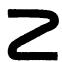
\includegraphics[keepaspectratio]{images/part002_287b28a9.jpg}}

Note that these functions are not continuous functions on T with compact support.

Let us pass to the definition of the integral.

PROPOSITION 16. --- There exists one and only one continuous linear mapping \(\mathbf{f} \mapsto \int \mathbf{f} d\mu\) , of the space \(\overline{\mathcal{L}}_{\mathrm{F}}^{1}(\mu)\) into \(\mathrm{F}\) , having the following property:

If \(\mathbf{f}\) is of the form \(t \mapsto g(t)\mathbf{a}\) , where \(\mathbf{a} \in \mathbf{F}\) , and where \(g\) is a positive function, finite, \(\mu\) -measurable and such that \(\mu^{\bullet}(g) < +\infty\) , then \(\int \mathbf{f} d\mu = \mu^{\bullet}(g) \cdot \mathbf{a}\) .

For, the semi-normed spaces \(\overline{\mathcal{L}}_{\mathrm{F}}^{1}(\mu)\) and \(\overline{\mathcal{L}}_{\mathrm{F}}^{1}(\mu')\) are identical. Since \(\mu^{\bullet} = \mu'^{\bullet}\) , the mapping \(\mathbf{f} \mapsto \int \mathbf{f} d\mu'\) satisfies the conditions of the statement. On the other hand, the set of functions of the form \(\mathbf{f} = g \cdot \mathbf{a}\) considered in the statement is total in \(\overline{\mathcal{L}}_{\mathrm{F}}^{1}(\mu')\) (Ch. IV, §3, No.~5, Prop. 10), whence uniqueness.

One says that \(\int f d\mu\) is the integral of f with respect to \(\mu\) , and this vector is also denoted \(\mu(\mathbf{f})\) or \(\int \mathbf{f}(t) d\mu(t)\) .

Since \(\int f d\mu = \int f d\mu'\) for every essentially integrable function f with values in F, all of the theory of the essential integral extends to measures on Hausdorff spaces, without new proofs; from it, one deduces results relative to the ordinary integral by restricting oneself to moderated functions. We cite in particular the following results:

--- Th. 3 of Ch. IV, §3, No.~4, its extension to \(\overline{\mathcal{L}}_{\mathrm{F}}^{p}\) , and its two corollaries.

--- Th. 4 of Ch. IV, §3, No.~5 (composition with a continuous linear mapping) and its corollaries; Props. 9, 11 and 12 of the same No.

--- All of the results of Ch. IV, §3, No.~6, relative to the ordered vector space structure of \(L^{p}\) .

--- All of the results of Ch. IV, §3, No.~7, and in particular Lebesgue's theorem.

--- All of the results of Ch. IV, §3, No.~8, on the relations between the spaces \(L_F^p\) .

--- Theorem 2 of Ch. IV, §4, No.~3 (the statement of Lebesgue's theorem specific to \(L_F^1\) ).

--- Hölder's inequality (Ch. IV, §6, No.~4, Th. 2) and its corollaries.

--- The relations between the spaces \(L_{F}^{p}\) established in Ch. IV, §6, No.~5.

-- The results on the duality of the spaces \(\mathbf{L}^p\) established in Ch. V, §5, No.~8.

--- The Dunford--Pettis theorem (Ch. VI, §2, No.~5, Th. 1), its Corollaries 1 and 2, and Prop. 10 of Ch. VI, §2, No.~6 (dual of \(L_{F}^{1}\) ).

\section{OPERATIONS ON MEASURES}

As in the preceding section, T denotes a Hausdorff topological space, and \(\mu\) a measure on T. Recall that all measures are assumed positive, absent mention to the contrary.

\subsection{Induced measure on a measurable subspace}

Let X be a subset of T, and let \(\nu\) be the restriction of the mapping \(\mu: K \mapsto \mu_{K}\) to the set of compact subsets of X; it is clear that \(\nu\) is a premeasure on X. On the other hand, let \(x \in X\) and let V be an open neighborhood of \(x\) in \(\mathbf{T}\) such that \(\mu^{\bullet}(\mathrm{V}) < +\infty\) ; then

\[
\nu^{\bullet}(\mathrm{X}\cap \mathrm{V}) = \sup_{\substack{\mathrm{K\ compact}\\ \mathrm{K}\subset \mathrm{X}\cap \mathrm{V}}}\mu^{\bullet}(\mathrm{K})\leqslant \mu^{\bullet}(\mathrm{V}) <   + \infty
\]

by Remark 3 of §1, No.~2, so that \(\nu\) is a measure.

When X is not \(\mu\) -measurable, the encumbrances \(\nu^{\bullet}\) and \((\mu^{\bullet})_{X}\) are not necessarily equal and the measure \(\nu\) presents no interest.

DEFINITION 1. --- Let X be a \(\mu\) -measurable subset of T. The restriction of \(\mu: \mathrm{K} \mapsto \mu_{\mathrm{K}}\) to the set of compact subsets of X is called the measure induced by \(\mu\) on the subspace X, and is denoted by \(\mu_{\mathrm{X}}\) or \(\mu|_{\mathrm{X}}\) .

PROPOSITION 1. --- Let X be a \(\mu\) -measurable subset of T. The encumbrance \((\mu_{\mathrm{X}})^{\bullet}\) is equal to the encumbrance \((\mu^{\bullet})_{\mathrm{X}}\) induced by \(\mu^{\bullet}\) on X (§1, No.~1). In other words, \((\mu_{\mathrm{X}})^{\bullet}(g) = \mu^{\bullet}(g^{0})\) for every function \(g \in \mathcal{F}_{+}(\mathrm{X})\) .

Let \(f \in \mathcal{F}_{+}(X)\) and let \(f^{0}\) be the extension by 0 of \(f\) to \(T\) . One has \((\mu^{\bullet})_{X}(f) = \mu^{\bullet}(f^{0}) = \sup_{L} \mu^{\bullet}(f^{0}\varphi_{L})\) , where \(L\) runs over the set of compact subsets of \(T\) (§1, No.~2, Prop. 2); similarly \((\mu_{X})^{\bullet}(f) = \sup_{K} \mu_{K}^{\bullet}(f_{K}) = \sup_{K} \mu^{\bullet}(f^{0}\varphi_{K})\) , where \(K\) runs over the set of compact subsets of \(X\) . Thus it all comes down to showing that \(\mu^{\bullet}(f^{0}\varphi_{L}) = \sup_{K} \mu^{\bullet}(f^{0}\varphi_{K})\) for every compact subset \(L\) of \(T\) , where \(K\) runs over the set of compact subsets of \(L \cap X\) . Now, let \((K_{n})\) be an increasing sequence of compact sets contained in \(L \cap X\) , such that \((L \cap X) - \bigcup_{n} K_{n}\) is locally \(\mu\) -negligible (§1, No.~8, Prop. 11); \(f^{0}\) being zero outside \(X\) , \(f^{0}\varphi_{L}\) is zero outside \(L \cap X\) hence is equal locally almost everywhere to the upper envelope of the sequence \((f^{0}\varphi_{K_{n}})\) . This implies that \(\mu^{\bullet}(f^{0}\varphi_{L}) = \sup \mu^{\bullet}(f^{0}\varphi_{K_{n}})\) , whence the desired result.

Remark 3). --- Let X be a \(\mu\) -measurable subset of T. By Prop. 10 of §1, No.~8, applied to \(g = \varphi_{\mathbf{X}}\) , there exists a crushing \((\mathrm{K}_{\alpha})_{\alpha \in \mathbf{A}}\) of T such that for each \(\alpha \in \mathbf{A}\) , either \(\mathrm{K}_{\alpha} \subset \mathrm{X}\) or \(\mathrm{K}_{\alpha} \subset \mathbb{C}\mathrm{X}\) . If one modifies the topology of T by the procedure of the Scholium of §1, No.~8, the space \(\mathrm{X}'\) obtained by equipping X with the topology induced by \(\mathrm{T}'\) is locally compact, and one knows how to associate to \(\mu\) (resp. to \(\mu_{\mathbf{X}}\) ) a measure \(\mu'\) (resp. \(\nu\) ) on \(\mathrm{T}'\) (resp. on \(\mathrm{X}'\) ) that admits the same essential upper integral as \(\mu\) (resp. \(\mu_{\mathbf{X}}\) ): this implies that \(\mu'_{\mathbf{X}'} = \nu\) . Since the locally negligible sets, measurable mappings, and essentially integrable functions with values in a Banach space, are the same for \(\mu\) and \(\mu'\) , and for \(\mu_{\mathbf{X}}\) and \((\mu_{\mathbf{X}})' = \nu = \mu'_{\mathbf{X}'}\) , the theory of integration with respect to an induced measure reduces to that which was treated in Ch. V, §7 in the special case of locally compact spaces. We leave to the reader the task of transcribing the results.
